\documentclass{article}

\usepackage{cancel}
\usepackage{tikz}
\usepackage{amsmath}
\usepackage{geometry}
\usepackage{graphicx}
\usepackage{amsfonts} 
\usepackage{verbatim}
\usepackage{mathrsfs}  
\usepackage{lmodern}
\usepackage{braket}
\usepackage{bookmark}
\usepackage{rotating}               % For rotatebox



\usetikzlibrary{petri, positioning, arrows.meta}
\hypersetup{
    colorlinks=true,
    linkcolor=black,
}

\tikzset{every transition/.style={draw,minimum width=1mm,minimum height=5mm},
         every place/.style={draw,thick,minimum size=6mm},
         instant/.style={draw, fill,minimum width=1mm,minimum height=5mm, inner sep=0pt},
        }

\renewcommand{\contentsname}{Indice}

\numberwithin{equation}{subsection}

\title{Appunti di Analisi dei Sistemi ad Eventi}
\author{Giacomo Sturm}
\date{AA: 2023/2024 - Ing. Informatica}

\begin{document}

\maketitle

\vspace{10mm}

\begin{center}
    Sorgente del file LaTeX disponibile su \url{https://github.com/00Darxk/Analisi-dei-Sistemi-ad-Eventi}
\end{center}

\clearpage

\tableofcontents

\clearpage

\section{Introduzione}

Verrano forniti due modelli di sistemi, reali o astratti, un modello matematico, reti di Code, ed un modello logico, reti di Petri. Quest'ultimo è un modello grafico, simile ad 
un diagramma di flusso. La rete di Petri analizza le interazioni tra gli elementi del sistema, mentre la rete di Code analizza nel tempo queste interazioni ingresso-uscita. 
In questi modelli si analizza l'evoluzione di una variabile di stato, da individuare nel sistema analizzato, per studiare la funzione obiettivo. La variazione della variabile 
di stato si studia tramite derivata continua o discreta, oppure si campiona il suo valore ad intervalli fissi. L'analisi ad eventi consiste nel misurare solamente se succede 
qualcosa al sistema, se avviene un evento, ovvero non c'è spreco di memoria campionando lo stesso valore. Per determinare un evento si controlla se la variabile di stato 
considerata è cambiata, questa variabile può essere sia deterministica oppure aleatoria. In caso sia aleatoria, conoscere la sua distribuzione di probabilità non è sufficiente 
per determinarne l'evouzione, sono necessaria la media, il valore centrale della distribuzione, e la varianza, la distanza dal valore centrale nella distribuzione. 



Si usano sistemi manufatturieri come esempi, poiché sono comuni e seplici da studiare. Viene definita una coda un luogo dove i clienti o utenti aspettano il servizio. Quando un 
cliente entra nel sistema, se è disponibile un servente, viene servito, se non è disponibile si mette in coda. Viene definito tempo di processamento il tempo 
necessario per un cliente affinché sia servito. Si considerano i clienti usciti dal sistema dopo essere stati serviti. Si considera per ipotesi la coda ordinate in FIFO (First 
In First Out), ovvero si considera il primo cliente entrato in coda, il primo servito, se sono disponibili serventi. La coda del modello può essere illimitata oppure 
limitata con un massimo numero clienti $k$. Si indica il numero dei serventi con $s$. Si definisce la variabile di stato di questo sistema il valore intero $n$ che 
rappresenta il numero di clienti all'interno del sistema, il suo valore massimo corrisponde alla massima capienza dei servneti e della coda: $n\in[0,s+k]$. Questo valore 
si incremente o decrementa di uno ogni volta che un cliente entra o esce dal sistema. In uno stesso istante non può avvenire più di un evento, ovvero la variabile può 
variare di uno in ogni istante. Si chiamano questi eventi di incremento e decremento processi di nascita e morte. Questo sistema è descritto da una legge di transizione:
\begin{equation*}
    \begin{cases}
        n=n+1\\
        n=n-1
    \end{cases}
\end{equation*}
Quest'equazione rappresenta la legge di evoluzione del sistema. Un evento rappresenta l'arrivo o la partenza di un cliente dal sistema. In questo modello la variazione è slegata 
dal tempo, noto solo il cambiamento della variabile di stato ad ogni evento, per cui rappresenta un modello logico. Se ad ogni evento viene assegnato una durata di tempo il 
modello diventa temporizzato, in maniera asincrona, ovvero ogni evento corrisponde ad intervalli di tempo diversi. L'obiettivo del modello è determinare l'evoluzione del sistema, 
questo può comprendere il numero di clienti, il tempo di servizio, differenza tra il tempo di entrata ed il tempo di uscita di un cliente, il tempo di attesa. Conoscendo il 
tempo di processamento si può deterinare se il sistemaè sotto o sovra-utilizzato.

\clearpage

\section{Reti di Petri}

La rete di Petri è un modello logico per rappresentare sistemi ad eventi deterministici (DES), può rappresentare comportamenti complessi come la sincronizzazione, il succedersi 
asincrono di eventi che avvengono in intervalli di tempo diversi, operazioni concorrenti che avvengono totalemente indipendentemente tra di loro, conflitti ed altre 
caratteristiche di sistemi ad eventi. 

La rete di petri è una rappresentazione grafica con una struttura matematica, è modulare e limitata, potendo rappresentare un ciclo continuo, è possibile gestire il ridimensionamento 
della rete senza perdere le sue proprietà. La rete è un grafo bipartito, formato da due tipi di nodi, i posti $p$ e le transizioni $t$. Si possono unire solamente posti-transizioni 
tramite archi orientati. 
\begin{center}
    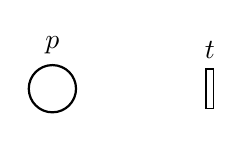
\begin{tikzpicture}
        \node[place, label=above:$p$](p)at(0,0){};
        \node[transition, label=above:$t$](t)at(2,0){};
    \end{tikzpicture}
\end{center}
Viene definito pre-set di un nodo $x$ l'insieme dei nodi immediatamente a monte di $x$: $\bullet x$, viene invece definito post-set di un nodo $x$ l'insieme dei nodi 
immediatamente a valle di $x$: $x\bullet$. Lo stato del sistema viene definito dalla marcatura $x$ un vettore colonna di dimensione pari al numero di posti $|P|$, dove $P$ 
indica l'insieme dei posti, ed avente ogni componente di valore uguale al numero di gettoni presenti nel posto associato:
\begin{equation*}
    x=\begin{pmatrix}
        x_1\\
        \vdots\\
        x_{|P|}
    \end{pmatrix}
\end{equation*}
Viene definita marcatura iniziale $x_0$ lo stato assunto dal sistema all'inizio della sua analisi. 
I nodi sono collegati da archi pesati, il peso di un arco esprime il numero di gettoni generati, in caso sia in entrata ad un posto, oppure consumati, in caso sia in entrata 
ad una transizione. Il peso di un arco può essere indicato come un numero espresso sopra l'arco, per convenzione se è omesso il peso si considera di peso unitario, oppure 
si possono rappresentare come un numero di archi pari al peso dell'arco:
\begin{center}
    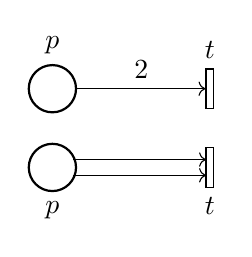
\begin{tikzpicture}
        \node[place, label=above:$p$](p1)at(0,0){};
        \node[transition, label=above:$t$](t1)at(2,0){};
        \draw[->](p1.0)--(t1.180)node[midway, above]{$2$};

        \draw[->](0.26,-0.9)--(1.95,-0.9);
        \draw[->](0.26,-1.1)--(1.95,-1.1);
        \node[place, label=below:$p$](p2)at(0,-1){};
        \node[transition, label=below:$t$](t2)at(2,-1){};
    \end{tikzpicture}
\end{center}

\subsection{Evoluzione}

Una transizione è abilitata se i posti a monte della transizione contengono almeno abbastanza gettoni da poter essere tutti consumati dai rispettivi archi. 

\begin{center}
    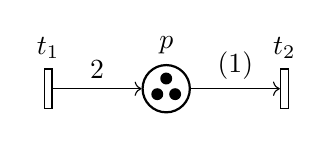
\begin{tikzpicture}
        \node[transition, label=above:$t_1$](t1)at(-0.5,0){};
        \node[place,tokens=3,label=above:$p$](p)at(1,0){};
        \node[transition,label=above:$t_2$](t2)at(2.5,0){};
        \draw[->](t1.0)--(p.180)node[midway, above]{$2$};
        \draw[->](p.0)--(t2.180)node[midway, above]{$(1)$};
    \end{tikzpicture}
\end{center}

In questo esempio la transizione $t_2$ è abilitata, poiché l'arco consuma tre gettoni e nel posto immediatamente a monte della transizione sono presenti tre gettoni. 
Ad ogni transizione può essere associato un tempo di processamento, in modo da temmporizzare il sistema. Se il pre-set di una transizione è vuoto, allora quella transizione 
è sempre abilitata. 

Il numero di stati possibili in una qualsiasi configurazione corrisponde al numero di transizioni abilitate in quella data configurazione. Questi stati possibili possono 
essere rappresentati con un grafo di stato, in base alla rete e alla marcatura iniziale considerata $x_0$. 

Si definiscono posti con un pre-set nullo appesi ed il numero di gettoni al loro interno può o rimanere costante o diminuire. Per cui se il sistema si basa solamente su posti 
appesi, allora sicuramente si bloccherà, incontra un "deadlock". 


L'evoluzione di un sistema viene determinata dall'accadimento di eventi abilitati, ognuno con una sua abilità di accadere. La possibilità che un evento accada dipende dall'
abilitazione di una transizione, l'effetto del suo accadimento corrisponde allo scatto di una transizione. L'abilitazione di una transizione dipende solamente dal peso dell'
arco in entrata e dai gettoni nel pre-set, è abilitata se il numero dei gettoni nel pre-set è almeno uguale al peso dei rispettivi archi. 
Lo scatto di una transizione provoca un "flusso" di gettoni, questo flusso non è continuo, poiché i gettoni in entrata alla transizione vengono consumati e ne vengono creati 
di nuovi sulla base del peso dell'arco in uscita, numero indipendente dal numero dei gettoni consumati. 

L'evoluzione comprende quattro passaggi ciclici: data una marcatura corrente si individua l'insieme delle transizioni abilitate, si sceglie casualmente, se non è specificato, 
una sola di queste transizioni, si provoca lo scatto di questa transizione che cambia la marcatura, si considera la nuova marcatura corrente e si ripetono questi passaggi. 

Una sequenza di transizioni, abilitate, $(t_1,\cdots,t_n)$ si esprime con il simbolo $S$. Questa sequenza rappresenta l'ordine con cui le transizioni scattano, affinché 
rappresenti una sequenza valida, le transizioni considerate devono essere abilitate quando è il loro turno di scattare. Diverse sequenze possono arrivare alla stessa 
marcatura. 
Un singolo posto può abilitare più di una transizione, ma dopo lo scatto di una delle transizioni abilitate, potrebbe non avere gettoni rimanenti per abilitare le altre. 

\subsection{Strutture Fondamentali}

Due transizioni si dicono in sequenza se sono collegate da un singolo posto:
\begin{center}
    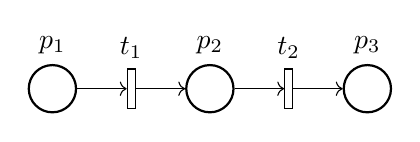
\begin{tikzpicture}
        \node[place, label=above:$p_1$](p1)at(0,0){};
        \node[transition, label=above:$t_1$](t1)at(1,0){};
        \node[place, label=above:$p_2$](p2)at(2,0){};
        \node[transition, label=above:$t_2$](t2)at(3,0){};
        \node[place, label=above:$p_3$](p3)at(4,0){};

        \draw[->](p1.0)--(t1.180);
        \draw[->](t1.0)--(p2.180);
        \draw[->](p2.0)--(t2.180);
        \draw[->](t2.0)--(p3.180);
    \end{tikzpicture}
\end{center}
Le transizioni $t_1$ e $t_2$ si dicono in sequenza. 


Un posto d'ingresso a due o più transizioni rappresenta un conflitto strutturale. Questo conflitto può essere effettivo se data una marcatura $M$, lo scatto di una transizione 
disabilita le altre transizioni. Il conflitto è potenziale se questo scatto non disabilita le altre transizioni. 
\begin{center}
    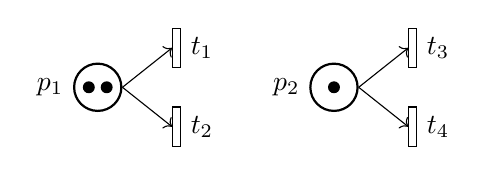
\begin{tikzpicture}
        \node[place, tokens=2, label=left:$p_1$](p1)at(0,0){};
        \node[transition, label=right:$t_1$](t1)at(1,0.5){};
        \node[transition, label=right:$t_2$](t2)at(1,-0.5){};

        \draw[->](p1.0)--(t1.180);
        \draw[->](p1.0)--(t2.180);

        \node[place, tokens=1, label=left:$p_2$](p2)at(3,0){};
        \node[transition, label=right:$t_3$](t3)at(4,0.5){};
        \node[transition, label=right:$t_4$](t4)at(4,-0.5){};

        \draw[->](p2.0)--(t3.180);
        \draw[->](p2.0)--(t4.180);
    \end{tikzpicture}
\end{center}
Le transizioni $t_1$ e $t_2$ si dicono in conflitto potenziale, le $t_3$ e $t_4$ si dicono in conflitto effettivo. 


Due, o più, transizioni si dicono concorrenti se la loro evoluzione è indipendente l'una dall'altra:
\begin{center}
    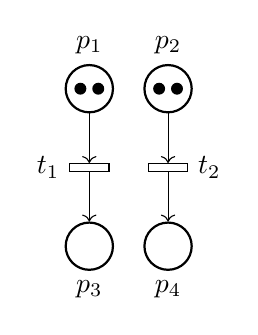
\begin{tikzpicture}
        \node[place, tokens=2, label=above:$p_1$](p1)at(0,0){};
        \node[place, tokens=2, label=above:$p_2$](p2)at(1,0){};
        \node[transition, rotate=90,label=above:$t_1$](t1)at(0,-1){};
        \node[transition, rotate=90,label=below:$t_2$](t2)at(1,-1){};
        \node[place, label=below:$p_3$](p3)at(0,-2){};
        \node[place, label=below:$p_4$](p4)at(1,-2){};

        \draw[->](p1.270)--(t1.0);
        \draw[->](p2.270)--(t2.0);
        \draw[<-](p3.90)--(t1.180);
        \draw[<-](p4.90)--(t2.180);
    \end{tikzpicture}
\end{center}
Le transizioni $t_1$ e $t_2$ si dicono in concorrenza strutturale, essendo entrambe abilitate si dicono in concorrenza effettiva. 



Due o più posti si dicono sincronizzati se come post-set presentano la stessa transizione:
\begin{center}
    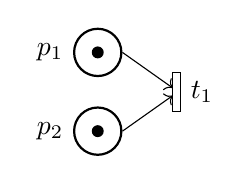
\begin{tikzpicture}
        \node[place, tokens=1, label=left:$p_1$](p1)at(0,0.5){};
        \node[place, tokens=1, label=left:$p_2$](p2)at(0,-0.5){};
        \node[transition, label=right:$t_1$](t1)at(1,0){};

        \draw[->](p1.0)--(0.95,0.05);
        \draw[->](p2.0)--(0.95,-0.05);
    \end{tikzpicture}
\end{center}
I posti $p_1$ e $p_2$ si dicono sincronizzati tra di loro, la transizione $t$ si identifica come transizione di sincronizzazione


Due o più posti si dicono concorrenti se presentano in pre-set la stessa transizione, per cui allo scatto di quella transizione vengono generati dei gettoni in entrambi i posti:
\begin{center}
    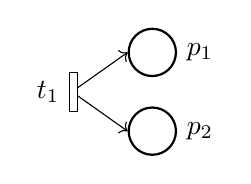
\begin{tikzpicture}
        \node[place, label=right:$p_1$](p1)at(1,0.5){};
        \node[place, label=right:$p_2$](p2)at(1,-0.5){};
        \node[transition, label=left:$t_1$](t1)at(0,0){};
        
        \draw[->](0.05,0.05)--(p1.180);
        \draw[->](0.05,-0.05)--(p2.180);
    \end{tikzpicture}
\end{center}
I due posti $p_1$ e $p_2$ si dicono concorrenti tra di loro, la transzizione $t$ si identifica come transizione di inizio concorrenza. 


Una rete di Petri si dice completa se non presenta nessun posto e transizione appese. 

\subsection{Esempio: Sistema Produttori/Consumatori}

Si considera un sistema semplice formato da uno o più produttori che creano oggetti e li depositano in un buffer condiviso da cui uno o più consumatori possono prelevarli 
e consumarli. Per rappresentare un consumatore o un produttore si un ciclo che produce uno o più gettoni e lo depositano in un posto esterno al ciclo, oppure  prelevano uno o 
più gettoni per poi consumarli con lo scatto di una transizione del ciclo:

\begin{center}
    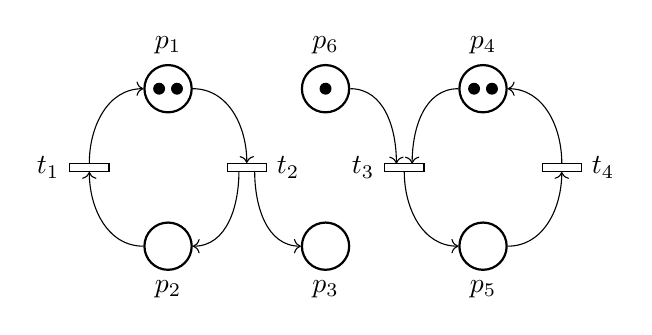
\begin{tikzpicture}
        \node[place, tokens=2, label=above:$p_1$](p1)at(0,1){};
        \node[place, label=below:$p_2$](p2)at(0,-1){};
        \node[transition, rotate=90, label=below:$t_2$](t2)at(1,0){};
        \node[transition, rotate=90, label=above:$t_1$](t1)at(-1,0){};
        \draw[->](p1.0)to [out=0,in=90](t2.0);
        \draw[->](0.9,-0.05)to [out=270,in=0](p2.0);
        \draw[->](p2.180)to [out=180,in=270](t1.180);
        \draw[->](t1.0)to [out=90,in=180](p1.180);

        \node[place, label=below:$p_3$](p3)at(2,-1){};
        \draw[->](1.1,-0.05)to[out=270,in=180](p3.180);
        
        \node[place, tokens=2, label=above:$p_4$](p4)at(4,1){};
        \node[place, label=below:$p_5$](p5)at(4,-1){};
        \node[transition, rotate=90, label=below:$t_4$](t4)at(5,0){};
        \node[transition, rotate=90, label=above:$t_3$](t3)at(3,0){};
        \draw[<-](p4.0)to [out=0,in=90](t4.0);
        \draw[<-](t4.180)to [out=270,in=0](p5.0);
        \draw[<-](p5.180)to [out=180,in=270](t3.180);
        \draw[<-](3.1,0.05)to [out=90,in=180](p4.180);

        \node[place, tokens=1,label=above:$p_6$](p6)at(2,1){};
        \draw[->](p6.0)to[out=0,in=90](2.9,0.05);
    \end{tikzpicture}
\end{center}

In questo caso ogni volta che la transizione $t_2$ scatta, viene generato un gettone nel posto $p_3$, quindi il ciclo rappresenta un ciclo di produttori ed il numero di 
gettoni nel ciclo, indica il numero di produttori. La transizione $t_3$ è abilitata solo se è presente almeno un gettone nel posto $p_6$, per cui questo ciclo 
consuma un gettone ogni volta che scatta $t_6$, rappresenta un ciclo di consumatori, ed il numero di gettoni nel ciclo rappresenta il numero di consumatori del sistema. 
In un qualsiasi ciclo il numero di gettoni rimane sempre costante, se il peso degli archi che generano gettoni è uguale al peso dei gettoni che consumano gettoni, e se le 
transizioni sono sempre abilitate, altrimenti il ciclo non potrebbe né consumare né generare gettoni. 

Per creare un sistema unico produttori-consumatori si considera un posto dove vengono depositati i gettoni generati dal ciclo dei produttori e consumati dal ciclo dei 
consumatori. Questo deposito può essere sia illimitato, nelle situazioni precedenti, oppure limitato. In questo caso è necessario un controllo nelle transizioni pre-set 
del buffer per impedire siano generatati gettoni se il deposito non può accomodarli, analogamente è necessario un controllo post-set per segnalare che un numero di gettoni è 
diminuito e quindi il deposito può accomodare più gettoni. Per indicare questo limite si crea un ciclo composto dalle transizioni generatrici nel cicli dei produttori, 
il posto buffer, le transizioni consumatrici dei cicli dei consumatori, ed un altro poste. In questo ciclo così definito il numero di gettoni rimane invariato, per cui il 
massimo numero di gettoni presenti nel deposito non può eccedere un limite imposto a priori:


\begin{center}
    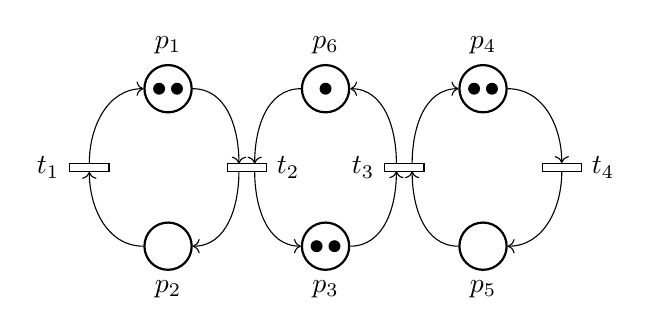
\begin{tikzpicture}
        \node[place, tokens=2, label=above:$p_1$](p1)at(0,1){};
        \node[place, label=below:$p_2$](p2)at(0,-1){};
        \node[transition, rotate=90, label=below:$t_2$](t2)at(1,0){};
        \node[transition, rotate=90, label=above:$t_1$](t1)at(-1,0){};
        \draw[->](p1.0)to [out=0,in=90](0.9,0.05);
        \draw[->](0.9,-0.05)to [out=270,in=0](p2.0);
        \draw[->](p2.180)to [out=180,in=270](t1.180);
        \draw[->](t1.0)to [out=90,in=180](p1.180);

        \node[place, tokens=2,label=below:$p_3$](p3)at(2,-1){};
        \draw[->](1.1,-0.05)to[out=270,in=180](p3.180);
        
        \node[place, tokens=2, label=above:$p_4$](p4)at(4,1){};
        \node[place, label=below:$p_5$](p5)at(4,-1){};
        \node[transition, rotate=90, label=below:$t_4$](t4)at(5,0){};
        \node[transition, rotate=90, label=above:$t_3$](t3)at(3,0){};
        \draw[->](p4.0)to [out=0,in=90](t4.0);
        \draw[->](t4.180)to [out=270,in=0](p5.0);
        \draw[->](p5.180)to [out=180,in=270](3.1,-0.05);
        \draw[->](3.1,0.05)to [out=90,in=180](p4.180);

        \node[place, tokens=1,label=above:$p_6$](p6)at(2,1){};
        \draw[<-](p6.0)to[out=0,in=90](2.9,0.05);
        \draw[->](p3.0)to[out=0,in=270](2.9,-0.05);
        \draw[->](p6.180)to[out=180,in=90](1.1,0.05);
    \end{tikzpicture}
\end{center}

In questo caso il deposito presenta un limite massimo di tre gettoni, e nel sistema sono presenti due consumatori e due produttori. Generalmente modelli di sistemi di produttori 
e consumatori presentano sempre dei cicli simili comunicanti tra di loro. 

\clearpage

\section{Proprietà}

Una stessa rete presenta proprietà diverse in base ad una diversa marcatura iniziale $M_0$. 

\subsection{Raggiungibilità}
Una marcatura $M^*$ si dice raggiugibile se esiste almeno una sequenza $S$ di transizioni abilitate tale che sia possibile, da una marcatura iniziale $M$, raggiungere la 
marcatura $M^*$:
\begin{equation*}
    M\left[S>M^*\right.
\end{equation*}


Si definisce, data una rete di Petri $N$ marcata con una marcatura $M_0$, l'insieme di raggiungibilità $R(N,M_0)$, l'insieme più piccolo di marcature tale che la marcatura 
iniziale appartiene all'insieme, e data una qualsiasi marcatura $M^*$ appartenente all'insieme, ed una qualsiasi transizione $t$, abilitata, appartenente all'insisme delle transizioni 
$T$ nella marcatura $M^*$. La transizione $M^{**}$ ottenuta facendo scattare la transizione $t$ nella marcatura $M^*$ anch'essa appartiene all'insieme di raggiungibilità. 
\begin{align*}
    &M_0\in R(N,M_0)\\
    &M^*\in R(N,M_0)\land t\in T\mbox{ t.c. } M^*\left[\right.t>M^{**}\implies M^{**}\in R(N,M_0)
\end{align*}

\subsection{Limitatezza}

Un posto $p_i$ di una rete $N$ si dice $k-$limitato se in tutte le marcature raggiungibili, da una marcatura iniziale $M_0$, quel posto presenta al massimo $k$ gettoni al 
suo interno:
\begin{equation*}
    \forall M\in R(N,M_0)\to m_i\leq k
\end{equation*} 
Una rete $N$ in una marcatura iniziale $M_0$ si dice $k-$limitata se tutti i suoi posti sono $k-$limitati. Se $k=1$, la rete si dice binaria, poiché ogni 
posto può avere o zero o un singolo gettone. Una rete si dice limitata al massimo numero di gettoni che possono esistere in uno dei suoi posti, per cui è sufficiente un 
singolo posto illimitato affinché l'intera rete sia illimitata. 

I cicli, analizzati precedentemente, rappresentano un caso semplice di rete limitata, poiché il numero di gettoni presenti nel ciclo rimane costante. 

\subsection{Reversibilità}

Una rete $N$ si dice reversibile, a partire da una marcatura iniziale $M_0$, se per ogni marcatura $M$ appartenente all'insieme di raggiungibilià, la marcatura iniziale 
appartiene all'insieme di raggiungibilità della marcatura $M$:
\begin{equation*}
    \forall M\in R(N,M_0)\implies M_0\in R(N,M)
\end{equation*}
Per cui una rete si dice reversibile se per ogni marcatura $M$ raggiungibile deve esistere una serie di scatti $S$ tali da ritornare alla marcatura originale $M_0$:
\begin{equation*}
    \forall M\in R(N,M_0)\implies M\left[\right.S>M_0
\end{equation*} 

\subsection{Conservatitivà}

Una rete $N$ con marcatura iniziale $M_0$ si dice conservativa in riferimento ad un vettore peso $W$ (colonna), maggiore uguale al vettore nullo $0$, di dimensione pari alla 
cardinalità dell'insieme dei posti $\mbox{dim} W=|P|$, se per ogni marcatura $M$ appartenente all'insieme di raggiungibilità $R$ il prodotto matriciale tra la trasposta del 
vettore peso $W$ ed il vettore marcatura $M$ assume un valore finito e costante:
\begin{equation*}
    \exists W\geq0\mbox{ t.c. }\forall M\in R(N,M_0)\implies W^T\cdot M=k\in\mathbb{R}^+
\end{equation*}


Il vettore peso $W$ poiché è maggiore uguale al vettore nullo presente al minimo una sola componente non nulla positiva, ed al massimo tutte componenti positive non nulle. Il 
prodotto tra $W^T$ e $M$ si può esprimere in diversi modi:
\begin{gather*}
    \forall M\in R(N,M_0):\,W^T\cdot M=\begin{pmatrix}
        w_1&\cdots&w_{|P|}
    \end{pmatrix}\cdot\begin{pmatrix}
        m_1\\
        \vdots\\
        m_{|P|}
    \end{pmatrix}=\displaystyle\sum_{j=1}^{|P|}w_jm_j=k\\
    M_0\in R(N,M_0)\implies W^T\cdot M=W^T\cdot M_0=k\\
    \displaystyle\sum_{j=1}^{|P|}w_jm_j=\sum_{j=1}^{|P|}w_jm_{j0}\to \sum_{j=1}^{|P|}w_j(m_j-m_{j0})=0
\end{gather*}


Una rete si dice conservativa, se esiste un vettore peso $W$ strettamente maggiore del vettore nullo, per cui il prodotto la trasposta del vettore ed una qualsiasi marcatura 
appartenente all'insieme di raggiungibilità risulta sempre costante:
\begin{equation*}
    \exists W>0\mbox{ t.c }\forall M\in R(N,M_0)\implies W^T\cdot M=k\in\mathbb{R}^+
\end{equation*}
Una rete conservativà quindi è $k-$limitata poiché non è necessario azzerare il contributo di un posto, a differenza del caso della conservativà in riferimento ad un vettore 
dove il vettore $W$ contiene tanti zeri quanti sono i posti illimitati nella rete $N$, in modo da azzerare i loro contriubti nella somma. 

Una rete si dice strettamente conservativa se è conservativa con riferimento al vettore identità, per cui tutte le componenti del vettore peso $W$ assumono valore unitario: 
$\forall j\in\,1,\cdots,|P|\implies w_j=1$. 


Una rete si dice non conservativa se è conservativa con riferimento ad un vettore peso nullo, per cui tutti i suoi posti sono illimitati, per cui il numero di posti rimane 
costante solo se non si considera nessun posto della rete. 

In generale per controllare la conservatività si cerca il sottoinsieme più grande dell'insieme dei posti della rete $N$ dove il numero di gettoni rimane complessivamente 
costante. Si deduce quindi che un ciclo rappresenta un elemeno conservativo, e se è presente in una rete, sarà sempre conservativà rispetto ad un vettore, se i posti del ciclo 
presentano almeno un vettore. 

\subsubsection{Vivezza}

Una transizione $t$, di una rete $N$ con marcatura iniziale $M_0$, si dice viva, se e solo se per ogni marcatura $M$ appartenente all'insieme di raggiungibilità $R$ esiste una 
marcaura $M^*$ raggiungibile da $M$, tale che la transizione $t$ sia abilitata:
\begin{equation*}
    t:\mbox{viva}\iff \forall M\in R(N,M_0),\,\exists M^*\in R(N,M)\mbox{ t.c. } t:\mbox{abilitata in }M^*
\end{equation*}
Una rete $N$, con marcatura iniziale $M_0$, si dice raggiungibile se e solo se tutte le sue transizioni $t_j$ sono vive:
\begin{equation*}
    N:\mbox{viva}\iff \forall t\in T\to t:\mbox{viva} 
\end{equation*}

\clearpage

\section{Analisi di Una Rete}

\subsection{Analisi Dinamica}

Partendo da una rete è possibile creare un grafo di stato o grafo di raggiungibilità, che racchiude le relazioni tra ogni marcatura appartenente all'insieme di raggiungibilità, 
data una marcatura iniziale $M_0$, tramite li scatti di una singola transizione. Questo grafo è sempre limitato, anche se la rete non lo è. Dal grafo è possible inferire sulle 
proprietà della rete in quella data configurazione. 
Bisogna tenere conto delle differenza tra le prorpietà strutturali di una rete, che non dipendono dalla marcatura iniziale $M_0$, e le proprietà dinamiche che dipedono dalla 
marcatura $M_0$. Le proprietà individuate da un'analisi strutturale sono più importanti poiché intrinseche alla rete e verrano studiate nelle sezioni successive. 

\subsubsection{Grafo di Raggiungibilità e di Copertura}

Un grafo di raggiungibilità è un grafo con un unico tipo di nodo che corrisponde ad una marcatura $M$. Sono presenti tanti nodi quante sono le marcature presenti nell'insieme 
di raggiungibilità $R$, a partire da una marcatura iniziale $M_0$. Gli archi del grafo uniscono due marcature collegate dallo scatto di una singola transizione, abilitata. 
Se è presente un numero finito di nodi, la rete è limitata, se sono presenti solo valori di $0$ e $1$, allora la rete è binaria. Se da ogni nodo del grafo esiste un percorso 
che abilita tutte le transizioni allora la rete è viva. Se da ogni nodo esiste un percorso che ritorna allo stesso nodo, la rete è reversibile. 
\\
Per costruire un grafo di raggiungibilità si parte dalla marcatura iniziale $M_0$, segnandola come nodo corrente. Si indica $M_k$ la marcatura associata al nodo corrente; 
se non ci sono più transizioni attivabili a partire dal nodo corrente, non considerate in precedenza rispetto allo stesso nodo, e se il nodo corrente non corrisponde alla 
marcatura iniziale $k>0$ allora si assegna come nodo corrente $M_{k-1}$, altrimeni l'algoritmo termina. Si considera la prima transizione abilitata, non considerata in precedenza 
con riferimento allo stesso nodo, e si calcola la marcatura raggiunta dal suo scatto. Se questa marcatura non corrisponde ad una marcatura già analizzata la si chiama $M_{k+1}$, 
e si crea un nodo associato ad essa collegato al nodo corrente da un arco, indicando la transizione scattata per arrivarci. Questo nodo diventa il nuovo nodo corrente e si 
ricomincia l'algoritmo cercando transizioni attivabili a partire da questo nodo corrente.  
\begin{center}
    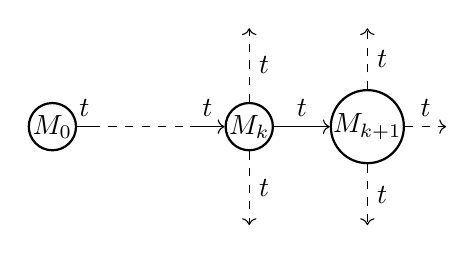
\begin{tikzpicture}
        \node[place](p1)at(-1,0){$M_0$};
        \draw[-](p1.0)--(-0.5,0)node[midway, above]{$t$};
        \draw[dashed](-0.5,0)--(0.75,0);

        \node[place](pk)at(1.5,0){$M_k$};
        \draw[->](0.75,0)--(pk.180)node[midway, above]{$t$};
        \draw[->, dashed](pk.90)--(1.5,1.25)node[midway, right]{$t$};
        \draw[->, dashed](pk.270)--(1.5,-1.25)node[midway, right]{$t$};
        

        \node[place](pk1)at(3,0){$M_{k+1}$};
        \draw[->](pk.0)--(pk1.180)node[midway, above]{$t$};
        \draw[->, dashed](pk1.90)--(3,1.25)node[midway, right]{$t$};
        \draw[->, dashed](pk1.270)--(3,-1.25)node[midway, right]{$t$};
        \draw[->, dashed](pk1.0)--(4,0)node[midway, above]{$t$};
    \end{tikzpicture}
\end{center}
Al termine di questo algoritmo si ottiene il grafo di raggiungibilità di una rete $N$ con marcatura iniziale $M_0$. 
Se tutti i nodi contengono marcatura, la cui somma dei gettoni è costante, allora la rete è strettamente conservativa, mentre se solo la somma di alcune posizioni delle 
marcature sono costanti allora la rete è conservativa in riferimento ad un vettore. Per controllare se la rete è conservativa rispetto ad un vettore $W>0$, bisogna controllare 
che la somma pesata assuma valore costante. Generalmente è meglio un vettore peso strettamente maggiore al vettore nullo che un vettore maggiore uguale al vettore nullo. 
Dato un vettore peso $W$, è possibile identificarne infiniti, combinazioni lineari del vettore $W$. 
\\
Se la rete è illimitata, si considera invece del grafo di raggiungibilità il grafo di copertura, che presenta un numero finito di nodi per poter descrivere la rete illimitata. 
Per identificare se una rete è illimitata si cerca una sequenza ammissibile di transizioni $S$ da una marcatura $M^*$ ad una marcatura $M^{**}$: $M^*\left[\right.S>M^{**}$, 
tale che la marcatura $M^{**}$ sia maggiore uguale alla marcatura $M^*$: $M^{**}\geq M^*$. Per cui presenta almeno un elemento maggiore della marcatura di partenza, ciò implica 
che il numero di gettoni complessivo è aumentato durante la sequenza $S$, ed almeno un posto presenta più gettoni rispetto all'inizio della sequenza. Necessariemente quindi la 
sequenza $S$ è abilitata nella nuova marcatura $M^{**}$, e può scattare portando ad un'altra marcatura $M^{***}$ maggiore uguale della precedente: 
$M^{**}\left[\right.S>M^{***}\mbox{ t.c. }M^{***}\geq M^{**}$. Continuando aribtrariamente questo processo è possibile aumentare il numero di gettoni all'interno di almeno un 
posto della rete, per cui quei posti sono illimitati. La posizione dei posti illimitati o strettamente maggiori si indica con il simbolo $\omega$, per indicare un numero 
arbitrario di gettoni:
\begin{equation*}
    M=\begin{pmatrix}
        \vdots\\
        \omega\\
        \vdots
    \end{pmatrix}
\end{equation*} 
Nel grafo di copertura, alla prima istanza di questo aumento arbitrario di gettoni si inserisce il termine $\omega$ nella posizione corrispondente ai 
posti illimitati, e si continua la costruzione del grafo seguendo le regole precedentemente definite. In alcuni casi è possibile, dato un determinato valore di $\omega$, 
svuotare il posto illimitato arrivando ad un nodo con una marcatura senza $\omega$. Oppure è possibile ritornare ad una marcatura finita precedentemente analizzata quindi 
collegando i due nodi con un'istruzione condizionale $\omega=k$, oltre al nome della transizione scattata. 
Se una rete è illimitata allora non può essere ciclica, ma può essere conservativa rispetto ad un vettore.

\subsubsection{Tecniche di Riduzione}

Si può ridurre il numero di posti di una rete, pur mantenendo le stesse proprietà, eccetto la conservatività. Poiché il vettore peso dipende dalla specifica rete considerata. 

Se due posti o due transizioni sono connessi in serie, avendo in comune una singola transizione o posto (vuoto), possono essere sotituiti da un singolo posto o transizione. 
In caso di transizioni poste in serie, si possono unire solo se il posto in comune tra di loro è vuoto, altrimenti si perderebbe l'informazione dei suoi gettoni, e se il peso 
dell'arco entrante al posto equivale al peso dell'arco uscente dal posto:
\begin{center}
    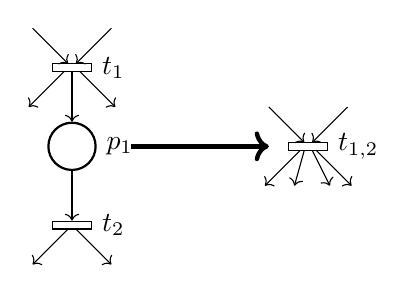
\begin{tikzpicture}
        \node[place, label=right:$p_1$](p)at(0,0){};
        \node[transition, rotate=90, label=below:$t_1$](t1)at(0,1){};
        \node[transition, rotate=90, label=below:$t_2$](t2)at(0,-1){};

        \draw[->](t1.180)--(p.90);
        \draw[->](p.270)--(t2.0);

        \draw[->](0.05,-1.05)--(0.5,-1.5);
        \draw[->](-0.05,-1.05)--(-0.5,-1.5);

        \draw[->](0.1,0.95)--(0.55,0.5);
        \draw[->](-0.1,0.95)--(-0.55,0.5);

        \draw[<-](0.05,1.05)--(0.5,1.5);
        \draw[<-](-0.05,1.05)--(-0.5,1.5);

        \draw[->, ultra thick](0.75,0)--(2.5,0);

        \node[transition, rotate=90, label=below:$t_{1,2}$](t3)at(3,0){};
        \draw[<-](3.05,0.05)--(3.5,0.5);
        \draw[<-](2.95,0.05)--(2.5,0.5);

        \draw[->](3.05,-0.05)--(3.275,-0.5);
        \draw[->](3.1,-0.05)--(3.55,-0.5);
        \draw[->](2.95,-0.05)--(2.825,-0.5);
        \draw[->](2.9,-0.05)--(2.45,-0.5);
    \end{tikzpicture}
\end{center}

Due posti si possono unire se sono collegati da un'unica transizione (abilitata), ed il peso degli archi entranti equivale il peso degli archi uscenti da essa. Il posto 
risultante contiene la somma dei gettoni presenti nei due posti:

\begin{center}
    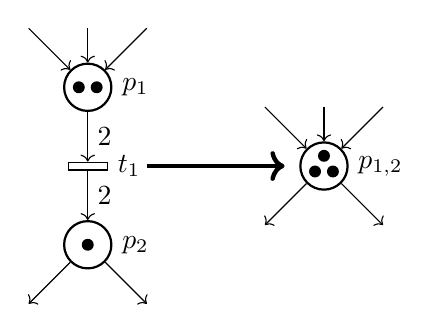
\begin{tikzpicture}
        \node[transition, rotate=90, label=below:$t_1$](t)at(0,0){};
        \node[place, tokens=2, label=right:$p_1$](p1)at(0,1){};
        \node[place, tokens=1, label=right:$p_2$](p2)at(0,-1){};

        \draw[->](p1.270)--(t.0)node[midway, right]{$2$};
        \draw[->](t.180)--(p2.90)node[midway, right]{$2$};

        \draw[->](0,1.75)--(p1.90);
        \draw[->](-0.75,1.75)--(p1.135);
        \draw[->](0.75,1.75)--(p1.45);

        \draw[->](p2.315)--(0.75,-1.75);
        \draw[->](p2.225)--(-0.75,-1.75);

        \draw[->, ultra thick](0.75,0)--(2.5,0);

        \node[place, tokens=3, label=right:$p_{1,2}$](p3)at(3,0){};

        \draw[->](3,0.75)--(p3.90);
        \draw[->](2.25,0.75)--(p3.135);
        \draw[->](3.75,0.75)--(p3.45);

        \draw[->](p3.315)--(3.75,-0.75);
        \draw[->](p3.225)--(2.25,-0.75);
    \end{tikzpicture}
\end{center}

Inoltre è possibile unire insieme transizioni o posti in parallelo, ovvero aventi gli stessi insieme di pre-set e post-set. 
In caso siano due posti connessi in parallelo, il posto risultante contiene la somma dei gettoni, mentre l'arco entrante al posto ha peso dato dalla somma dei pesi degli 
archi entranti nei due posti originali, analogamente per l'arco uscente dal posto risultante:
\begin{center}
    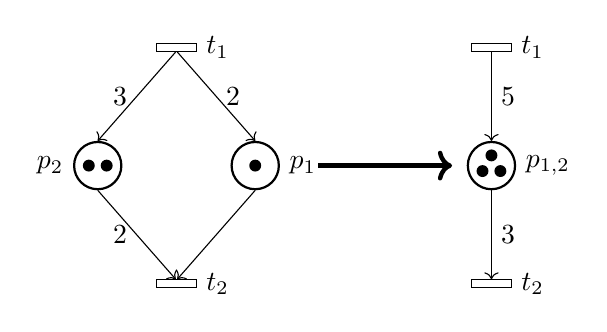
\begin{tikzpicture}
        \node[transition, rotate=90, label=below:$t_1$](t1)at(0,1.5){};
        \node[transition, rotate=90, label=below:$t_2$](t2)at(0,-1.5){};
        \node[place, tokens=1, label=right:$p_1$](p1)at(1,0){};
        \node[place, tokens=2, label=left:$p_2$](p2)at(-1,0){};

        \draw[->](t1.190)--(p1.90)node[midway, right]{$2$};
        \draw[->](t1.170)--(p2.90)node[midway, left]{$3$};
        \draw[<-](t2.350)--(p1.270)node[midway, right]{};
        \draw[<-](t2.10)--(p2.270)node[midway, left]{$2$};
        
        \draw[->,ultra thick](1.8,0)--(3.5,0);

        \node[transition, rotate=90, label=below:$t_1$](t3)at(4,1.5){};
        \node[transition, rotate=90, label=below:$t_2$](t4)at(4,-1.5){}; 
        \node[place, tokens=3, label=right:$p_{1,2}$](p3)at(4,0){};
        
        \draw[->](t3.180)--(p3.90)node[midway, right]{$5$};
        \draw[->](p3.270)--(t4.0)node[midway, right]{$3$};
    \end{tikzpicture}
\end{center}

In caso siano presenti due transizioni poste in parallelo, per unirle è necessario che gli archi entranti in entrambe le transizioni abbiano lo stesso peso, analogamente per 
le transizioni in uscita, in questo modo date due marcatura prima e dopo lo scatto di una delle due transizioni è impossibile distinguere quale delle due sia scattata, per cui 
si considerano come un'unica transizione:
\begin{center}
    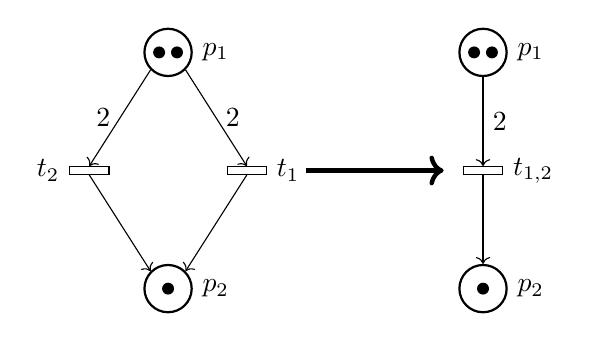
\begin{tikzpicture}
        \node[transition, rotate=90, label=below:$t_1$](t1)at(1,0){};
        \node[transition, rotate=90, label=above:$t_2$](t2)at(-1,0){};
        \node[place, tokens=2, label=right:$p_1$](p1)at(0,1.5){};
        \node[place, tokens=1, label=right:$p_2$](p2)at(0,-1.5){};

        \draw[->](p1.315)--(t1.0)node[midway, right]{$2$};
        \draw[->](p1.225)--(t2.0)node[midway, left]{$2$};
        \draw[->](t1.180)--(p2.45);
        \draw[->](t2.180)--(p2.135);

        \draw[->,ultra thick](1.75,0)--(3.5,0);

        \node[transition, rotate=90, label=below:$t_{1,2}$](t3)at(4,0){};
        \node[place, tokens=2, label=right:$p_1$](p3)at(4,1.5){};
        \node[place, tokens=1, label=right:$p_2$](p4)at(4,-1.5){};
        
        \draw[->](p3.270)--(t3.0)node[midway, right]{$2$};
        \draw[->](t3.180)--(p4.90);
    \end{tikzpicture}
\end{center}

Se in una rete è presente un autociclo, ovvero un posto o una transizione che presenta in pre-set e post-set lo stesso insieme, si può eliminare poiché non altera il 
comportamento della rete. 
In caso sia un posto in autociclo, se gli archi in entrata ed in uscita al posto hanno lo stesso peso, il numero di gettoni al suo interno rimane costante; se il peso dell'arco 
in entrata alla transizione è maggiore del numero dei gettoni interni al posto, la rete è morta, poiché quella transizione non sarà mai abilitata, quindi eliminandolo bisogna 
indicare che la rete sia morta, anche se la rete ridotta non lo è. Se il peso dell'arco in uscita è minore del peso dell'arco in entrata si raggiunge la stessa situazione, e 
la transizione diventa morta. 
\begin{center}
    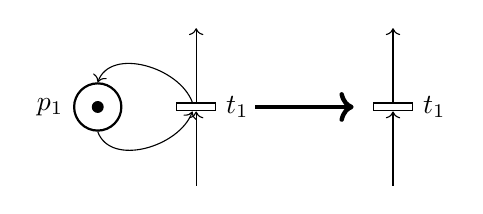
\begin{tikzpicture}
        \node[place, tokens=1, label=left:$p_1$](p1)at(0.25,0){};
        \node[transition, rotate=90, label=below:$t_1$](t1)at(1.5,0){};

        \draw[->](t1.40)to[out=110,in=70](p1.90);
        \draw[<-](t1.140)to[out=250,in=290](p1.270);

        \draw[->](1.5,-1)--(t1.180);
        \draw[->](t1.0)--(1.5,1);

        \draw[->,ultra thick](2.25,0)--(3.5,0);

        \node[transition, rotate=90, label=below:$t_1$](t2)at(4,0){};
        \draw[->](4,-1)--(t2.180);
        \draw[->](t2.0)--(4,1);
    \end{tikzpicture}
\end{center} 

Analogamente se è presenta una transizione avente in pre-set ed in post-set lo stesso posto, se il posto è $k-$limitato ed il peso del'arco entrante nella transizione è maggiore 
di $k$, allora quella transizione è morta. Se il peso degli archi entranti ed uscenti dalla transizione è uguale, non altera il numero dei gettoni nel posto associato. 
\begin{center}
    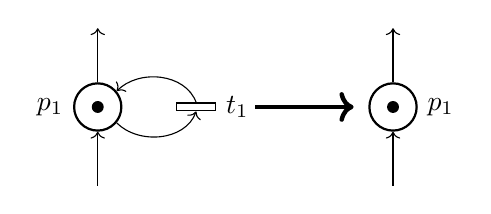
\begin{tikzpicture}
        \node[place, tokens=1, label=left:$p_1$](p1)at(0.25,0){};
        \node[transition, rotate=90, label=below:$t_1$](t1)at(1.5,0){};

        \draw[->](t1.0)to[out=110,in=45](p1.40);
        \draw[<-](t1.180)to[out=250,in=315](p1.320);

        \draw[->](0.25,-1)--(p1.270);
        \draw[->](p1.90)--(0.25,1);

        \draw[->,ultra thick](2.25,0)--(3.5,0);

        \node[place, tokens=1, label=right:$p_1$](t2)at(4,0){};
        \draw[->](4,-1)--(t2.270);
        \draw[->](t2.90)--(4,1);
    \end{tikzpicture}
\end{center} 
Gli autociclici possono essere espressi come una doppia freccia, invece di due archi separati, quando entrambi i pesi uguali. 

\subsection{Rappresentazione Algebrica}

Una qualsiasi rete di petri può essere rappresentata in riferimento a $3$ matrici:


La matrice di ingresso $I$ (Input) è una matrice avente tante righe quanti sono i posti nella rete e tante colonne quante sono le transizioni. Gli elemnenti della matrice 
sono interi positivi o nulli: $I\in M(|P|,|T|,\mathbb{N})$. L'elemento $i_{ij}$ della matrice $I:=(i_{ij})$ viene definito come il peso dell'arco che collega il $i-$esimo posto 
alla $j-$esima transizione. Per cui questa matrice racchiude tutti i pesi degli archi entranti nelle transizioni. 

Analogamente la matrice di uscita $O\in M(|P|,|T|,\mathbb{N})$ (Output), contiene tutti i pesi degli archi uscenti dalle transizioni. L'elemento $o_{ij}$ della matrice $O:=(o_{ij})$ 
è definito come il peso dell'arco uscente dalla transizione $j$ in entrata al posto $i$. 


La matrice di incidenza $C$ è definita come la differenza tra la matrice di uscita e la matrice di entrata:
\begin{equation*}
    C:=O-I\in M(|P|,|T|,\mathbb{Z})
\end{equation*}

Se nella rete è presente un ciclo, a gettoni costanti, le componenti della matrice di incidenza relative a quegli archi assumono valori nulli. Se un elemento $c_{ij}$ della 
matrice di incidenza $C:=(c_{ij})$ è negativo, allora la transizione $t_j$ è in ingresso al posto $p_i$, se è positivo allora la transizione $t_j$ è di uscita dal posto $p_i$, 
ed il modulo dell'elemento indica il peso dell'arco corrispondente. 


Questa rappresentazione corrisponde ad un'analisi puramente strutturale di una rete, poiché si perdono le informazioni sui gettoni contenuti nei posti. Se ogni elemento 
della matrice di incidenza è nullo, allora la rete è strettamente, strutturalmente, conservativa, poiché è indipendente dalla marcatura $M_0$ della rete. Gli elementi della 
matrice di incidenza possono essere nulli in caso sia presente un ciclo o un autociclo nelle rispettive posizioni. Una rete senza autocicli si definisce pura. 


Per determinare se una data transizione $t_i$ è abilitata, si controlla se il vettore marcatura corrente $M$ è maggiore uguale alla colonna $i-$esima della matrice di ingresso 
$I_i$, poiché quella colonna indica quanti gettoni devono essere consumati per lo scatto della transizione $t_i$ e se la marcatura $M$ è maggiore uguale a quella colonna, 
sono presenti necessariamente abbastanza gettoni per scattare la transizione $t_i$ in tutti i posti collegati, rendendola abilitata:
\begin{equation*}
    t_i:\mbox{ abilitata }\iff M\geq I_i
\end{equation*}
La marcatura corrente $M$ se viene sommata con la colonna $i-$esima della matrice di uscita risulta maggiore uguale di $M$ prima della somma, poiché gli elementi della matrice 
$O$ sono strettamente positivi, allora:
\begin{gather*}
    M+O_i\geq M\geq I_i\to M+O_i\geq I_i\\
    M+O_i-I_i=M+C_i\geq 0
\end{gather*}
La marcatura $M$ rappresenta lo stato della rete, mentre l'espressione $M+C_i$ rappresenta l'equazione di stato della rete, ovvero la sua evoluzione dopo lo scatto di una 
transizione $t_i$, se abilitata. Rappresenta una nuova marcatura raggiunta dalla rete aggiungendo e togliendo gettoni in base ai pesi degli archi entranti ed uscenti alla 
transizione $t_i$. L'evoluzione della rete non dipende dalla marcatura, ma dipende interamente dalla topo logia della stessa. Per ottenere la colonna $i-$esima della matrice 
di incidenza si considera il versore $s_i$, vettore di dimensione pari alla cardinalità dell'insieme delle transizioni $\mbox{dim }s=|T|$, avente tutti elementi nulli eccetto 
per l'elemento nella posizione $i-$esima:
\begin{equation*}
    s_i=\begin{pmatrix}
        0\\
        \vdots\\
        1\\
        \vdots\\
        0
    \end{pmatrix}\begin{matrix}
        (1)\\
        \vdots\\
        (i)\\
        \vdots\\
        (|T|)
    \end{matrix}
\end{equation*}
Per cui si può esprimere una colonna corrispondente ad una transizione $t_i$ attraverso il prodotto della matrice di incidenza per il versore associato a quella transizione:
\begin{equation*}
    C_i=C\cdot s_i
\end{equation*} 

Una sequenza di scatti $S=t_{k_1},\cdots,t_{k_n}$ abilitata in una marcatura iniziale $M_0$ è una sequenza di transizioni $t_{k_j}\in T,\;\forall j=1,\cdots,n$ tali che la 
marcatura raggiunta dallo scatto di $t_{k_j}$ da $M_j$ porta ad una marcatura $M_{j+1}$ dove la transizione $t_{k_{j+1}}$ è abilitata:
\begin{equation*}
    M_0\left[\right.t_{k_1}>M_1,\cdots,M_{n-1}\left[\right.t_{k_n}>M_n\implies M_0\left[\right.t_{k_1},\cdots,t_{k_n}=S>M_n
\end{equation*}

Una sequenza di transizioni $S$ si dice sequenza di scatti solo se tutte le transizioni sono abilitate quando devono scattare, non necessariamente vero per una sequenza 
arbitraria. Se questo è verificato la sequenza di transizioni si dice ammissibile. 

L'effetto di una sequenza di scatti $S=t_{k_1},\cdots,t_{k_n}$ da una marcatura $M_0$ ad una marcatura $M^*$ può essere espresso mediante l'equazione di stato della rete:
\begin{equation*}
    M^*=M+C_{k_1}+\cdots+C_{k_n}=M+C\cdot(s_{k_1}+\cdots+c_{k_n})
\end{equation*}
Si definisce il vettore colonna $s_k$, di dimensione pari alla cardinalità dell'insieme delle transizioni, associato alla sequenza di scatti, che indica quante volte ogni 
singola transizione è scattata, senza fornire informazioni sull'ordine in cui le transizioni scattano. Presenta nella posizione $i-$esima il valore corrispondente al numero 
di occorrenze della transizione $t_i$ nella sequenza $S$:
\begin{equation*}
    s_{k_1}+\cdots+s_{k_n}=s_k
\end{equation*}
Per cui si può esprimere l'evoluzione della rete da una marcatura $M_0$ dopo una sequenza di scatti $S$ come:
\begin{equation*}
    M_0\left[\right.S>M^*:\;\;M^*=M_0+C\cdot s_k
\end{equation*}
Quest'espressione indica una relazione lineare. 

\subsection{Analisi Strutturale}

L'analisi della rappresentazione algebrica di una rete permette di trovare proprietà esclusivamente strutturali, intrinseche alla rete. Quest'analisi si basa solo su 
informazioni contenute nel grafo di incidenza. Questa analisi punta ad individuare delle strutture specifiche nella rete. Alcune di queste strutture si chiamano invarianti, 
possono essere di posto, $P-$invarianti, di transizione, $T-$invarianti. 


Si dicono invarianti canonici, se il minimo comune multiplo dei loro elementi è pari ad uno, per trovare l'invariante più grande si sommano tutti gli invarianti più piccoli 
trovati. 
Si definisce il supporto di un invariante $||x||$, l'insieme di elementi associati alla rete corrispondenti ai componenti del vettore $x$. 
Un invariante si dice a supporto minimo se il suo supporto non contiente il supporto di altri invarianti.   
Generalemente quando si risolvono i sistemi associati agli invarianti, se è possibile scegliere, ai componenti si assegnano i valori nulli altrimenti $1$, per trovare quelli a 
supporto minimo e canonici. Gli invarianti sia a supporto minimo che canonici formano una base dell'insieme degli invarianti della rete. 


\subsubsection{P-invarianti}

Gli invarianti di posto sono delle strutture associate all'insieme dei posti $P$, dove la somma pesata dei gettoni è costante, si studiano per determinare la conservatività 
strutturale della rete. Un $P-$invariante di una rete $N$ viene definito come un vettore colonna $x$ di dimensione pari alla cardinalità dell'insieme dei posti $|P|$, tale 
che il prodotto matriciale tra la sua trasposta ed una qualsiasi marcatura $M$ raggiungibile da $M_0$ è costante e finito:
\begin{equation*}
    x^TM=x^TM_0,\;\forall M\in R(N,M_0)
\end{equation*} 

Per calcolare i $P-$invarianti si considera una generica marcatura raggiungibile $M$ da una sequenza di scatti $S$, con associato un vettore $s$:
\begin{equation*}
    M=M_0+Cs
\end{equation*}
Gli ivarianti di posto $x$ sono tali che:
\begin{equation*}
    x^TM=x^T(M+Cs)=x^TM_0+Csx^T
\end{equation*}
Per definizione $x^TM=x^TM_0$, allora, un vettore colonna $x$ si dice $P-$invariante se rispetta la seguente equazione:
\begin{equation*}
    x^TCs=0
\end{equation*}
Per definizione un vettore associato ad una sequenza di scatti $S$ non è nullo, per cui non si considera come soluzione $s=0$. Per cui il l'equazione diventa un sistema 
di $|P|$ equazioni: 
\begin{equation*}
    x^TC=0\to\begin{pmatrix}
        x_1 & \cdots & x_{|P|}
    \end{pmatrix}\cdot\begin{pmatrix}
        c_{11} & \cdots & c_{1|T|}\\
        \vdots & \ddots & \vdots\\
        c_{|P|1} & \cdots & c_{|P||T|}
    \end{pmatrix}=\begin{pmatrix}
        0\\
        \vdots\\
        0
    \end{pmatrix}\to\begin{cases}
        x_1c_{11}+\cdots+x_{|P|}c_{|P|1}=&0\\
        \vdots &\vdots\\
        x_1c_{1|T|}+\cdots+x_{|P|}c_{|P||T|}=&0
    \end{cases}
\end{equation*}
Si omette la soluzione $x$ uguale al vettore nullo, poiché inutile nell'analisi di una rete di Petri. Le soluzioni accettate sono vettori colonna con componenti intere. Se 
non sono presenti soluzioni oppure se le componenti dell'invariante sono minori o uguali a $0$: $x\leq0$, la rete non è strutturalmente conservativa, se è presente almeno una 
soluzione è possibile crearne infinite tramite combinazione lineare e la rete è strutturalmente conservativa. Se il $P-$invariante è tale che $x\geq0$ la rete è conservativa 
rispetto a quel vettore peso, se è strettamente positivo, la rete è strutturalmente conservativa, se il vettore corrisponde al vettore identità, la rete si dice strettamente 
strutturalmente conservativa.  

\subsubsection{T-invarianti}

I $T-$invarianti sono analoghi ai $P-$invarianti associati alle transizioni $T$. Un vettore colonna $y$, di dimensione pari alla cardinalità dell'insieme delle transizioni, 
si definisce $T-$invariante, se dopo lo scatto delle transizioni indicate dal vettore si ritorna alla marcatura iniziale, quindi esprime la reversibilità della rete. 
Si considera uno sequenza di scatti $S: M_0\left[\right.S>M_0$ associata al vettore $y$: 
\begin{equation*}
    M=M_0+Cy=M_0\to Cy=0
\end{equation*}
Non si considera $y=0$ una soluzione, per cui un vettore colonna si definisce $T-$invariante se non è il vettore nullo e ha componenti interi. Per trovare 
le componenti del vettore $y$ bisogna risolvare un sistema di $|T|$ equazioni: 
\begin{gather*}
    Cy=0\to
    \begin{pmatrix}
        c_{11} & \cdots & c_{1|T|}\\
        \vdots & \ddots & \vdots\\
        c_{|P|1} & \cdots & c_{|P||T|}
    \end{pmatrix}\cdot
    \begin{pmatrix}
        y_1\\
        \vdots\\
        y_{|T|}
    \end{pmatrix}=
    \begin{pmatrix}
        0\\
        \vdots\\
        0
    \end{pmatrix}\to
    \begin{cases}
        y_1c_{11}+\cdots+y_{|T|}c_{1|T|}=&0\\
        \vdots & \vdots\\
        y_{|T|}c_{|P|1}+\cdots+y_{|T|}c_{|P||T|}=&0
    \end{cases}
\end{gather*}
Se il vettore $y$ è maggiore uguale del vettore nullo, ovvero ha componenti tutte positive, la rete si dice reversibile, altrimenti se presenta almeno una componente negativa 
implicherebbe che per ritornare alla marcatura iniziale bisognerebbe invertire lo scatto di una transizione, ma ciò è impossibile, quindi in questo caso la rete non è 
reversibile. Se una ammete un $T-$invariante, ne ammette infiniti. Se non ammette $T-$invarianti sicuramente non è reversibile. Bisogna comunque verificare che la sequenza di 
scatti indicata dal $T-$invariante sia abilitata, per dimostrare che la rete è reversibile. 

\clearpage

\section{Modellazione di Un Sistema}

Si modellano sistemi produttivi per la loro semplicità, poiché sono facilmente intuibili. In questi sistemi un materiale grezzo subisce delle lavorazioni fino a diventare un 
prodotto finito. Per modellare un sistema vengono fornite le informazioni sui passaggi che il grezzo attraversa nel sistema, sulla base di queste informaizoni si 
modellano le varie parti. 

In generale un sistema produttivo è formato da varie risorse, macchine per la lavorazione, dispositivi per lo spostamento dei materiali, e dei depositi dove conservare 
i materiali. Ogni passaggio effettuato dal grezzo richiede l'uso di almeno una risorsa disponibile, poiché possono essere impegnate da altri compiti. Le azioni associate a 
questi passaggi vengono espresse come gli eventi del sistema. 


Bisogna tenere conto delle condizioni che permettono lo scatto di una transizione, ovvero l'accadimento di un evento nel sistema. 
Per cui tutte le risorse vengono rappresentate come dei cicli, poiché se una risorsa è limitata, il sistema produttivo si blocca, ed è necessario un modo per modellare una 
risorsa che non si esaurisce, ciò viene quindi rappresentato come un ciclo in una rete di Petri. L'uso di un ciclo permette anche di modellare la disponibilatà di una 
risorsa per effettuare una serie di eventi.  

\subsection{Elementi Fondamentali}

Ad ogni evento viene associata una transizione temporizzata, che rappresenta la possibilità accada un evento, mentre gli stati di una risorsa sono associati a posti collegati 
alle rispettive transizioni. Gli stati 
associati ai posti forniscono informazioni sulla disponibilità di un evento e di una o più risorse, possono esprimere che un evento sta accadendo, informano il sistema 
quando l'attività è conclusa, e restituiscono le risorse usate per quell'evento al termine dell'attività. Ogni attività è rappresentata da un ciclo, per indicare la 
disponibilità delle risorse utilizzare, e per esprimere i passaggi che compie il grezzo tramite quelle risorse. Quindi per definire una serie di eventi, si segue il 
percorso di un generico materiale grezzo e si associano tutti gli eventi a rispettive transizioni, con pre-set e post-set determinati dal comportamento del sistema, per ogni 
possibile percorso che il materiale può attraversare nel sistema, senza saltare passaggi. In questo modo si analizzano algoritmicamente tutte le possibili interazioni tra le 
risorse presenti nel sistema. Quando un materiale esce dal sistema, non deve essere più considerato nella costruzione del modello. Ogni evento del sistema può richiedere 
un certo intervallo di tempo per il suo accadimento, per cui deveno essere associati a rispettive transizioni temporizzate. Per cui è necessario distinguere nella rete tra le 
transizioni istantanee e quelle temporizzate. Si indicano le transizioni temporizzate come dei blocchi vuoti, mentre quelle istantanee sono rappresentate come delle barrette. Se 
è noto l'intervallo di una transizione temporizzata $\tau$, viene inserito dentro la transizione:
\begin{center}
    \begin{tikzpicture}
        \node[transition,rotate=90,label=above:$t_1$](t3)at(-2,0){\rotatebox{-90}{$\,\tau\,$}};
        \node[transition,rotate=90,label=above:$t_2$](t1)at(0,0){};
        \node[instant,rotate=90,label=below:$t_3$](t2)at(2,0){};
        \draw[->](-2,1)--(t3.0);
        \draw[->](t3.180)--(-2,-1);
        \draw[->](0,1)--(t1.0);
        \draw[->](t1.180)--(0,-1);
        \draw[->](2,1)--(t2.0);
        \draw[->](t2.180)--(2,-1);
    \end{tikzpicture}
\end{center}
La transizione $t_1$ è temporizzata, con associato un intervallo di tempo non necessariamente noto, mentre la transizione $t_2$ è istantanea, ovvero l'evento associato avviene in un itervallo di 
tempo tendente a zero. 
Le marcature in un posto vengono consumate da una transizione solamente al termine dell'intervallo di tempo associato ad essa. 

In caso alcune risorse sono sempre disponibili, possono essere rappresentate con un transizione istantanea appesa a monte, oppure con un autociclo, rappresentabile come una 
doppia freccia: 
\begin{center}
    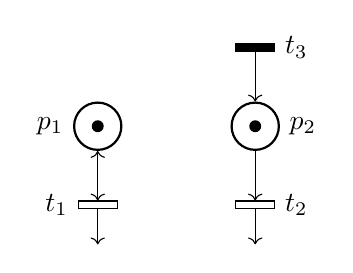
\begin{tikzpicture}
        \node[place,tokens=1,label=left:$p_1$](p1)at(0,0){};
        \node[place,tokens=1,label=right:$p_2$](p2)at(2,0){};
        \node[transition,rotate=90,label=above:$t_1$](t1)at(0,-1){};
        \node[transition,rotate=90,label=below:$t_2$](t2)at(2,-1){};
        \node[instant,rotate=90,label=below:$t_3$](t3)at(2,1){};

        \draw[<->](p1.270)--(t1.0);
        \draw[->](t1.180)--(0,-1.5);

        \draw[->](t3.180)--(p2.90);
        \draw[->](p2.270)--(t2.0);
        \draw[->](t2.180)--(2,-1.5);
    \end{tikzpicture}
\end{center}

Entrambe queste rappresentazioni esprimono lo stessa risorsa sempre disponibile, ma in caso siano presenti transizioni appese nella rete, si perde la limitatezza, per cui è 
preferibile usare un autociclo. Altrimenti una risorsa può essere disponibile al passare di un intervallo di tempo finito, in questo caso si modella tramite una 
transizione temporizzata posta a monte. Se la risorsa non è capacitata ad $1$, si può modellare come un autociclo di peso pari ai gettoni necessari marcato sufficientemente, 
oppure con una transizione a monte, ma ciò rende la rete illimitata. La disponibilità di una risorsa si esprime tramite un posto, che presenta in pre-set la transizione che 
determina la fine dell'uso di quella risorsa, mentre in post-set la transizione che determina l'inizio dell'uso della risorsa. Per cui lo stato del posto indica se la risorsa 
è disponibile, oppure è occupata da un'attività:
\begin{center}
    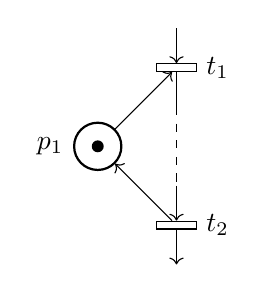
\begin{tikzpicture}
        \node[transition, rotate=90,label=below:$t_1$](t1)at(0,2){};
        \node[transition, rotate=90,label=below:$t_2$](t2)at(0,0){};
        \node[place, tokens=1, label=left:$p_1$](p1)at(-1,1){};

        \draw[-](t1.180)--(0,1.5);
        \draw[dashed](0,1.5)--(0,0.5);
        \draw[->](0,0.5)--(t2.0);
        \draw[->](t2.45)--(p1.315);
        \draw[->](p1.45)--(t1.135);
        \draw[->](0,2.5)--(t1.0);
        \draw[->](t2.180)--(0,-0.5);
    \end{tikzpicture}
\end{center}

\subsection{Conflitto Strutturale}

Quando è presente una risorsa condivisa nel sistema, il posto associato può creare un conflitto strutturale in caso non sia modellato correttamente. Se il posto è in entrata 
a due transizioni temporizzate, poiché i gettoni vengono consumati solo dopo l'intervallo di tempo della transizione, è possibile che abiliti entrambi le transizioni ed 
entrambi lavorino usando lo stesso numero di gettoni, ciò non corrisopnde alla realtà. Poiché una volta che una risorsa è usata in processo, non può essere usata contemporaneamente 
in un altra attività. Per cui per rappresentare una risorsa condivisa, si usano delle transizioni istantane prima delle transizioni temporizzate, per indicare che la 
risorsa non è più disponibile, ed è impegnata da una delle attività, in questo modo l'altra transizione in entrata non è più abilitata. Questo conflitto diventa quindi solo 
potenziale: 
\begin{center}
    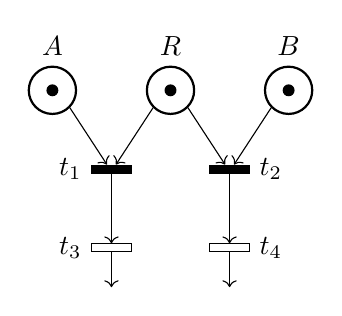
\begin{tikzpicture}
        \node[place, tokens=1,label=above:$A$](a)at(-0.5,0){};
        \node[place, tokens=1,label=above:$R$](r)at(1,0){};
        \node[place, tokens=1,label=above:$B$](b)at(2.5,0){};
        \node[instant,rotate=90,label=above:$t_1$](t1)at(0.25,-1){};
        \node[instant,rotate=90,label=below:$t_2$](t2)at(1.75,-1){};
        \node[transition,rotate=90,label=above:$t_3$](t3)at(0.25,-2){};
        \node[transition,rotate=90,label=below:$t_4$](t4)at(1.75,-2){};

        \draw[->](a.315)--(t1.45);
        \draw[->](r.225)--(t1.315);
        \draw[->](r.315)--(t2.45);
        \draw[->](b.225)--(t2.315);
        \draw[->](t1.180)--(t3.0);
        \draw[->](t2.180)--(t4.0);
        \draw[->](t3.180)--(0.25,-2.5);
        \draw[->](t4.180)--(1.75,-2.5);
    \end{tikzpicture}
\end{center}

Se non viene specificato, il conflitto non viene risolto, ovvero non si modella quale delle due o più transizioni ha la precedenza. Generalmente, se è presente una 
lavorazione in parallelo, con delle risorse condivise, è più efficiente richiedere la disponibilità della risorsa condivisa, all'inizio della lavorazione, in modo da 
non aspettare la sua disponibilità, e bloccare il resto del processo. 

\subsection{Esempio: Cella di Assemblatura}

In generale le macchine come tutte le risorse reali sono capacitate, per cui vanno modellate come un ciclo, marcato. All'inizio di ogni modello, bisogna marcare i cicli di 
produzione e lavorazione, per permettere al sistema di operare. 

Si considera una cella di assemblatura, dove due materiali grezzi $A$ e $B$ vengono inseriti nel sistema tramite rulli trasportatori. All'interno della cella è presente un 
braccio meccanico, capacitato ad uno, che può spostare i grezzi in due diverse macchine di lavorazione, una per ogni grezzo $M_A$ e $M_B$, anch'esse capacitate ad uno. 
Quando entrambe le macchine hanno processato un grezzo, possono essere raccolte dal braccio meccanico ed assemblate in un prodotto finito. Prima che il robot posso traspostare 
altri materiali grezzi, deve spostare il prodotto finito in un buffer di output, capacitatato ad uno, prima che il prodotto possa essere traspostato all'esterno del sistema. 

In questo caso ogni risorsa è capacitata ad uno, per cui il robot all'inizio può prendere uno dei due grezzi, per cui è presente un conflitto strutturale all'inizio. Si 
modella senza risolvere il conflitto. Se il robot prendere un grezzo quando entrambe le macchine hanno processato sono occupate con un grezzo il sistema si blocca, per cui 
bisogna modellare il sistema in modo da impedire questo "deadlock". 

Si considerano i materiali grezzi sempre disponibili nel sistema, per cui si rappresentano come degli autocicli, legati a monte della transizione, istantanea, per attivare 
una delle due sequenza di lavorazione $A$ e $B$. Gli eventi che avvengono processando uno dei due grezzi sono gli stessi tra di loro, per cui si può modellare uno solo di 
questi processi ed includere una sua copia per rappresentare l'altro, fino alla fine della lavorazione del grezzo nella macchina apposita. Quindi si rappresenta una 
rete, in parte simmetrica. 


Se il robot è disponibile $R$, il grezzo è disponibile $A/B$, e la macchina è disponibile $M_A/M_B$, allora può cominciare la fase di lavorazione del grezzo. Si rappresenta 
come $3$ posti a monte di una transizione istantanea $t_{R_A}/t_{R_B}$, poiché è presente un conflitto strutturale con l'altrs sequenza di lavorazione dell'altro grezzo:
\begin{center}
    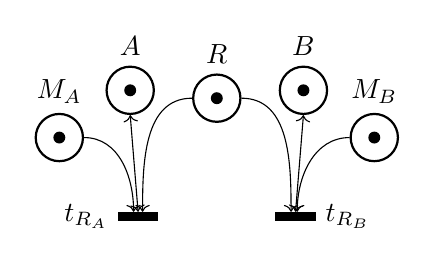
\begin{tikzpicture}
        \node[place,tokens=1,label=above:$M_A$](ma)at(0,0){};
        \node[place,tokens=1,label=above:$A$](a)at(0.9,0.6){};
        \node[place,tokens=1,label=above:$R$](r)at(2,0.5){};
        \node[place,tokens=1,label=above:$B$](b)at(3.1,0.6){};
        \node[place,tokens=1,label=above:$M_B$](mb)at(4,0){};
        \node[instant, rotate=90, label=above:$t_{R_A}$](tra)at(1,-1){};
        \node[instant, rotate=90, label=below:$t_{R_B}$](trb)at(3,-1){};

        \draw[->](ma.0)to[out=0, in=90](tra.45);
        \draw[<->](a.270)--(tra.0);
        \draw[->](r.180)to[out=180,in=90](tra.315);
        \draw[->](r.0)to[out=0,in=90](trb.45);
        \draw[->](mb.180)to[out=180, in=90](trb.340);
        \draw[<->](b.270)--(trb.0);
    \end{tikzpicture}
\end{center}
Le transizioni istantanee portano ad un posto $R_A/R_B$, che esprime lo stato del braccio meccanico, occupato nel carico $A/B.pick$, traporto $A/B.mov$ e scarico $A/B.release$ 
del grezzo $A$ o $B$, e rappresentano il primo evento nella sequenza della lavorazione della macchina. Ognuna delle operazioni del braccio viene espressa come una transizione 
temporizzata, e solo al termine, ovvero allo scarico $t_{A/B.release}$, il braccio torna di nuovo disponibile allo spostamento di un altro grezzo. 
\begin{center}
    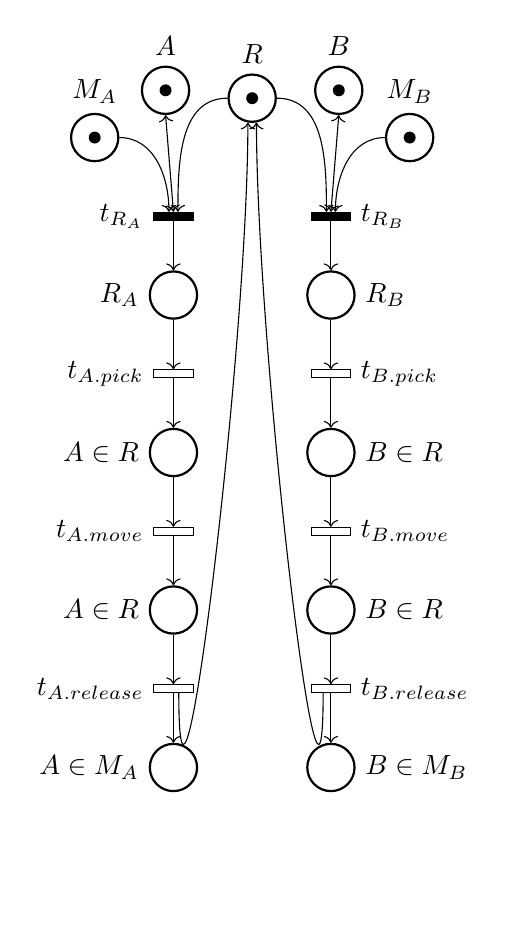
\begin{tikzpicture}
        \node[place,tokens=1,label=above:$M_A$](ma)at(0,0){};
        \node[place,tokens=1,label=above:$A$](a)at(0.9,0.6){};
        \node[place,tokens=1,label=above:$R$](r)at(2,0.5){};
        \node[place,tokens=1,label=above:$B$](b)at(3.1,0.6){};
        \node[place,tokens=1,label=above:$M_B$](mb)at(4,0){};
        \node[instant, rotate=90, label=above:$t_{R_A}$](tra)at(1,-1){};
        \node[instant, rotate=90, label=below:$t_{R_B}$](trb)at(3,-1){};

        \draw[->](ma.0)to[out=0, in=90](tra.45);
        \draw[<->](a.270)--(tra.0);
        \draw[->](r.180)to[out=180,in=90](tra.315);
        \draw[->](r.0)to[out=0,in=90](trb.45);
        \draw[->](mb.180)to[out=180, in=90](trb.315);
        \draw[<->](b.270)--(trb.0);

        \node[place,tokens=0,label=left:$R_A$](ra)at(1,-2){};
        \node[place,tokens=0,label=right:$R_B$](rb)at(3,-2){};
        \node[transition, rotate=90, label=above:$t_{A.pick}$](rap)at(1,-3){};
        \node[transition, rotate=90, label=below:$t_{B.pick}$](rbp)at(3,-3){};
        \node[place,tokens=0,label=left:$A\in R$](ra1)at(1,-4){};
        \node[place,tokens=0,label=right:$B\in R$](rb1)at(3,-4){};
        \node[transition, rotate=90, label=above:$t_{A.move}$](ram)at(1,-5){};
        \node[transition, rotate=90, label=below:$t_{B.move}$](rbm)at(3,-5){};
        \node[place,tokens=0,label=left:$A\in R$](ra2)at(1,-6){};
        \node[place,tokens=0,label=right:$B\in R$](rb2)at(3,-6){};
        \node[transition, rotate=90, label=above:$t_{A.release}$](rar)at(1,-7){};
        \node[transition, rotate=90, label=below:$t_{B.release}$](rbr)at(3,-7){};
        \node[place,tokens=0,label=left:$A\in M_A$](maa)at(1,-8){};
        \node[place,tokens=0,label=right:$B\in M_B$](mbb)at(3,-8){};

        \draw[->](tra.180)--(ra.90);
        \draw[->](ra.270)--(rap.0);
        \draw[->](rap.180)--(ra1.90);
        \draw[->](ra1.270)--(ram.0);
        \draw[->](ram.180)--(ra2.90);
        \draw[->](ra2.270)--(rar.0);
        \draw[->](rar.180)--(maa.90);

        \draw[->](trb.180)--(rb.90);
        \draw[->](rb.270)--(rbp.0);
        \draw[->](rbp.180)--(rb1.90);
        \draw[->](rb1.270)--(rbm.0);
        \draw[->](rbm.180)--(rb2.90);
        \draw[->](rb2.270)--(rbr.0);
        \draw[->](rbr.180)--(mbb.90);

        \draw[->](rar.230)to[out=270,in=270](r.260);
        \draw[->](rbr.120)to[out=270,in=270](r.280);
    \end{tikzpicture}
\end{center}
Le transizioni in sequenza $t_{A/B.pick},\;t_{A/B.move},\;t_{A/B.release}$ possono essere sostituite da un'unica transizione associata ad un intervallo di tempo pari alla 
somma dei tre intervalli delle transizioni originali:
\begin{center}
    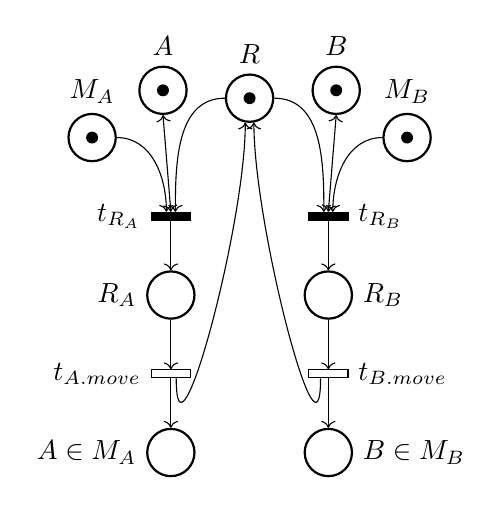
\begin{tikzpicture}
        \node[place,tokens=1,label=above:$M_A$](ma)at(0,0){};
        \node[place,tokens=1,label=above:$A$](a)at(0.9,0.6){};
        \node[place,tokens=1,label=above:$R$](r)at(2,0.5){};
        \node[place,tokens=1,label=above:$B$](b)at(3.1,0.6){};
        \node[place,tokens=1,label=above:$M_B$](mb)at(4,0){};
        \node[instant, rotate=90, label=above:$t_{R_A}$](tra)at(1,-1){};
        \node[instant, rotate=90, label=below:$t_{R_B}$](trb)at(3,-1){};

        \draw[->](ma.0)to[out=0, in=90](tra.45);
        \draw[<->](a.270)--(tra.0);
        \draw[->](r.180)to[out=180,in=90](tra.315);
        \draw[->](r.0)to[out=0,in=90](trb.45);
        \draw[->](mb.180)to[out=180, in=90](trb.315);
        \draw[<->](b.270)--(trb.0);

        \node[place,tokens=0,label=left:$R_A$](ra)at(1,-2){};
        \node[place,tokens=0,label=right:$R_B$](rb)at(3,-2){};
        \node[transition, rotate=90, label=above:$t_{A.move}$](rap)at(1,-3){};
        \node[transition, rotate=90, label=below:$t_{B.move}$](rbp)at(3,-3){};
        \draw[->](tra.180)--(ra.90);
        \draw[->](ra.270)--(rap.0);
        \draw[->](trb.180)--(rb.90);
        \draw[->](rb.270)--(rbp.0);
        \draw[->](rap.230)to[out=270,in=270](r.260);
        \draw[->](rbp.120)to[out=270,in=270](r.280);

        \node[place,tokens=0,label=left:$A\in M_A$](maa)at(1,-4){};
        \node[place,tokens=0,label=right:$B\in M_B$](mbb)at(3,-4){};
        \draw[->](rap.180)--(maa.90);
        \draw[->](rbp.180)--(mbb.90);
    \end{tikzpicture}
\end{center}

Quando le macchine presenta al loro interno un grezzo, lo lavorano fino ad un prodotto finito, quest'operazione viene rappresentata come una transizione 
temporizzata $t_{A/B.make}$ che passa dallo stato $A/B\in M_{A/B}$ allo stato $A_f/B_f\in M_{A/B}$, entrambi espressi come posti. Quando entrambi i posti che rappresentano 
lo stato del prodotto finito in una macchina sono marcati, ed il braccio meccanico è disponibile, allora il braccio può raccogliere entrambi i prodotti finiti per cominciare 
il processo di assemblaggio finale. Quest'operazione si rappresenta mediante una transizione $t_{R_{(A_f,B_f)}}$ istantanea, poiché lo stesso braccio è in entrata ad altre due 
transizioni, ma il conflitto non avverrà mai con questa transizione, poiché può essere abilitata se e solo se le due transizioni in ingresso alle sequenze di lavorazione dei 
grezzi sono disabilitate. Questo perché in ogni ciclo di lavorazione di un grezzo è presente un singolo gettone, che abilita solo una transizione. 
Questa transizione porta ad uno stato $R_{(A_f,B_f)}$, ovvero la sequenza di assemblaggio finale. Il braccio meccanico quindi raccogli i due prodotti finiti da $M_A$ e $M_B$, 
rendendoli nuovamente disponibili, e arriva ad uno stato $(A_f,B_f)\in R$, dove entrambi i prodotti finiti sono all'interno del robot munito di braccio meccanico. 

\begin{center}
    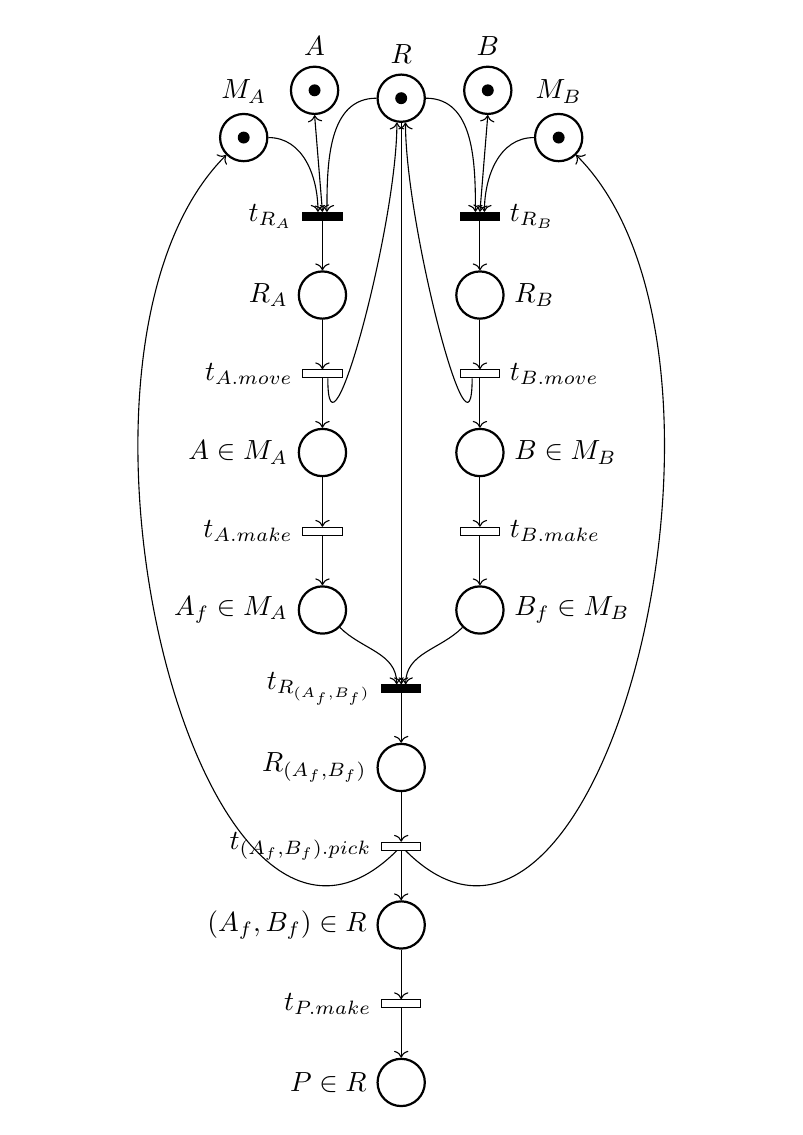
\begin{tikzpicture}
        \node[place,tokens=1,label=above:$M_A$](ma)at(0,0){};
        \node[place,tokens=1,label=above:$A$](a)at(0.9,0.6){};
        \node[place,tokens=1,label=above:$R$](r)at(2,0.5){};
        \node[place,tokens=1,label=above:$B$](b)at(3.1,0.6){};
        \node[place,tokens=1,label=above:$M_B$](mb)at(4,0){};
        \node[instant, rotate=90, label=above:$t_{R_A}$](tra)at(1,-1){};
        \node[instant, rotate=90, label=below:$t_{R_B}$](trb)at(3,-1){};

        \draw[->](ma.0)to[out=0, in=90](tra.45);
        \draw[<->](a.270)--(tra.0);
        \draw[->](r.180)to[out=180,in=90](tra.315);
        \draw[->](r.0)to[out=0,in=90](trb.45);
        \draw[->](mb.180)to[out=180, in=90](trb.315);
        \draw[<->](b.270)--(trb.0);

        \node[place,tokens=0,label=left:$R_A$](ra)at(1,-2){};
        \node[place,tokens=0,label=right:$R_B$](rb)at(3,-2){};
        \node[transition, rotate=90, label=above:$t_{A.move}$](rap)at(1,-3){};
        \node[transition, rotate=90, label=below:$t_{B.move}$](rbp)at(3,-3){};
        \draw[->](tra.180)--(ra.90);
        \draw[->](ra.270)--(rap.0);
        \draw[->](trb.180)--(rb.90);
        \draw[->](rb.270)--(rbp.0);
        \draw[->](rap.230)to[out=270,in=270](r.260);
        \draw[->](rbp.120)to[out=270,in=270](r.280);

        \node[place,tokens=0,label=left:$A\in M_A$](maa)at(1,-4){};
        \node[place,tokens=0,label=right:$B\in M_B$](mbb)at(3,-4){};
        \draw[->](rap.180)--(maa.90);
        \draw[->](rbp.180)--(mbb.90);

        \node[transition, rotate=90, label=above:$t_{A.make}$](amake)at(1,-5){};
        \node[transition, rotate=90, label=below:$t_{B.make}$](bmake)at(3,-5){};
        \node[place,tokens=0,label=left:$A_f\in M_A$](maf)at(1,-6){};
        \node[place,tokens=0,label=right:$B_f\in M_B$](mbf)at(3,-6){};

        \draw[->](maa.270)--(amake.0);
        \draw[->](amake.180)--(maf.90);
        \draw[->](mbb.270)--(bmake.0);
        \draw[->](bmake.180)--(mbf.90);
        
        \node[instant, rotate=90,label=above:$t_{R_{(A_f,B_f)}}$](rabf)at(2,-7){};
        \draw[->](r.270)--(rabf.0);
        \draw[->](maf.315)to[out=315, in=90](rabf.45);
        \draw[->](mbf.225)to[out=225, in=90](rabf.315);

        \node[place,label=left:$R_{(A_f,B_f)}$](rf)at(2,-8){};
        \draw[->](rabf.180)--(rf.90);
        \node[transition, rotate=90,label=above:$t_{(A_f,B_f).pick}$](trf)at(2,-9){};
        \node[place,tokens=0,label=left:${ (A_f, B_f)\in R}$](ttrf)at(2,-10){};
        \draw[->](rf.270)--(trf.0);
        \draw[->](trf.180)--(ttrf.90);
        
        \draw[->](trf.135)to[out=225,in=225](ma.225);
        \draw[->](trf.225)to[out=315,in=315](mb.315);
        
        \node[transition, rotate=90,label=above:$t_{P.make}$](trp)at(2,-11){};
        \node[place,tokens=0,label=left:${P\in R}$](rp)at(2,-12){};

        \draw[->](ttrf.270)--(trp.0);
        \draw[->](trp.180)--(rp.90);
    \end{tikzpicture}
\end{center}

A questo 
punto si rappresenta l'assemblaggio finale come una transizione temporizzata $t_{P.make}$, che porta allo stato $P\in R$, dove $P$ denota il prodotto finale, contenuto ancora 
nel robot. Il prodotto finito viene riposto nel buffer di uscita $O$, se è disponibile, rendendo nuovamente disponibile il robot per spostare altri grezzi. Il prodotto finito 
nel buffer finale a questo punto viene trasportato fuori dal sistema, modellato con un altra transizione temporizzata $t_{P.out}$:

\begin{center}
    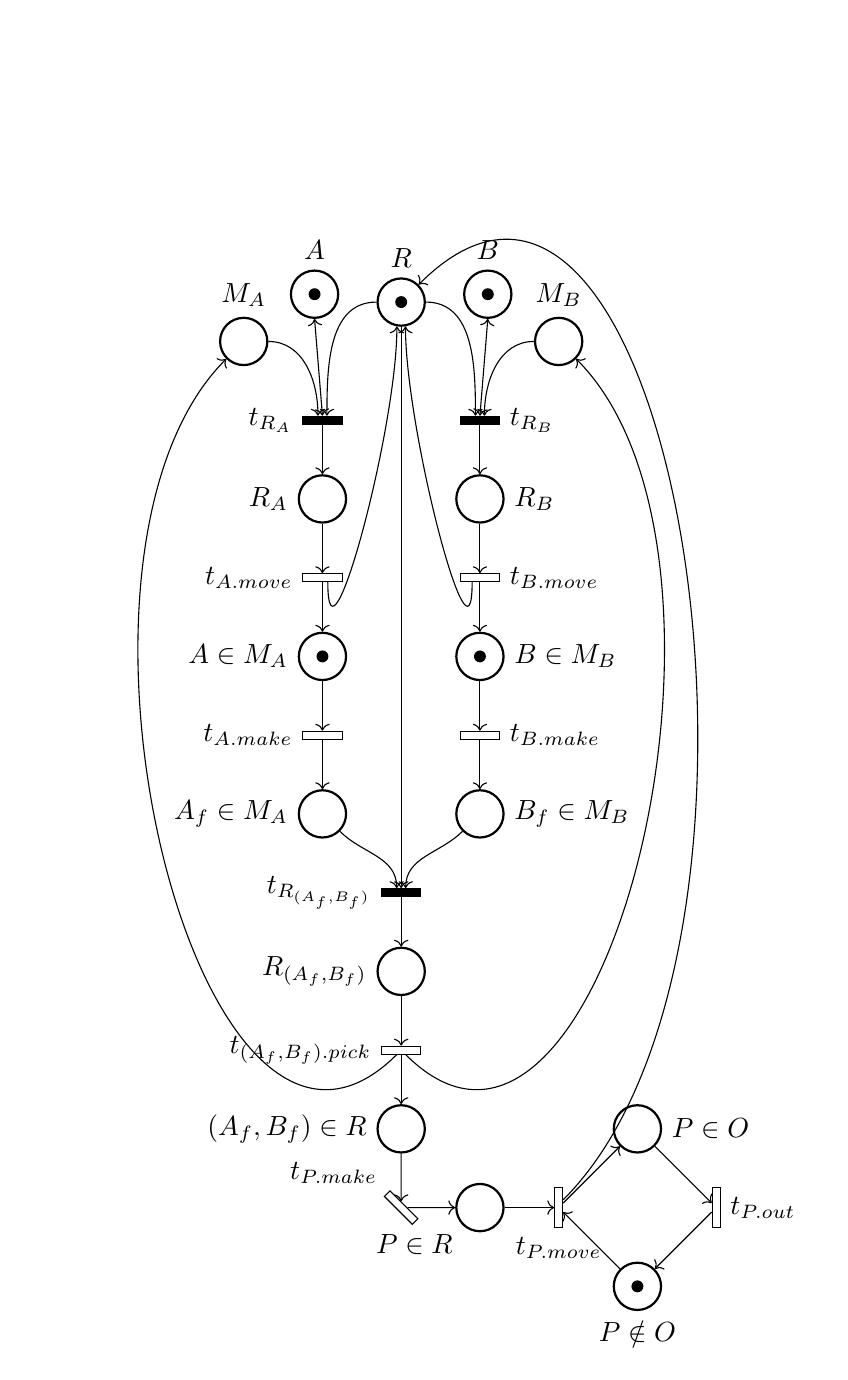
\begin{tikzpicture}
        \node[place,tokens=0,label=above:$M_A$](ma)at(0,0){};
        \node[place,tokens=1,label=above:$A$](a)at(0.9,0.6){};
        \node[place,tokens=1,label=above:$R$](r)at(2,0.5){};
        \node[place,tokens=1,label=above:$B$](b)at(3.1,0.6){};
        \node[place,tokens=0,label=above:$M_B$](mb)at(4,0){};
        \node[instant, rotate=90, label=above:$t_{R_A}$](tra)at(1,-1){};
        \node[instant, rotate=90, label=below:$t_{R_B}$](trb)at(3,-1){};

        \draw[->](ma.0)to[out=0, in=90](tra.45);
        \draw[<->](a.270)--(tra.0);
        \draw[->](r.180)to[out=180,in=90](tra.315);
        \draw[->](r.0)to[out=0,in=90](trb.45);
        \draw[->](mb.180)to[out=180, in=90](trb.315);
        \draw[<->](b.270)--(trb.0);

        \node[place,tokens=0,label=left:$R_A$](ra)at(1,-2){};
        \node[place,tokens=0,label=right:$R_B$](rb)at(3,-2){};
        \node[transition, rotate=90, label=above:$t_{A.move}$](rap)at(1,-3){};
        \node[transition, rotate=90, label=below:$t_{B.move}$](rbp)at(3,-3){};
        \draw[->](tra.180)--(ra.90);
        \draw[->](ra.270)--(rap.0);
        \draw[->](trb.180)--(rb.90);
        \draw[->](rb.270)--(rbp.0);
        \draw[->](rap.230)to[out=270,in=270](r.260);
        \draw[->](rbp.120)to[out=270,in=270](r.280);

        \node[place,tokens=1,label=left:$A\in M_A$](maa)at(1,-4){};
        \node[place,tokens=1,label=right:$B\in M_B$](mbb)at(3,-4){};
        \draw[->](rap.180)--(maa.90);
        \draw[->](rbp.180)--(mbb.90);

        \node[transition, rotate=90, label=above:$t_{A.make}$](amake)at(1,-5){};
        \node[transition, rotate=90, label=below:$t_{B.make}$](bmake)at(3,-5){};
        \node[place,tokens=0,label=left:$A_f\in M_A$](maf)at(1,-6){};
        \node[place,tokens=0,label=right:$B_f\in M_B$](mbf)at(3,-6){};

        \draw[->](maa.270)--(amake.0);
        \draw[->](amake.180)--(maf.90);
        \draw[->](mbb.270)--(bmake.0);
        \draw[->](bmake.180)--(mbf.90);
        
        \node[instant, rotate=90,label=above:$t_{R_{(A_f,B_f)}}$](rabf)at(2,-7){};
        \draw[->](r.270)--(rabf.0);
        \draw[->](maf.315)to[out=315, in=90](rabf.45);
        \draw[->](mbf.225)to[out=225, in=90](rabf.315);

        \node[place,label=left:$R_{(A_f,B_f)}$](rf)at(2,-8){};
        \draw[->](rabf.180)--(rf.90);
        \node[transition, rotate=90,label=above:$t_{(A_f,B_f).pick}$](trf)at(2,-9){};
        \node[place,tokens=0,label=left:${ (A_f, B_f)\in R}$](ttrf)at(2,-10){};
        \draw[->](rf.270)--(trf.0);
        \draw[->](trf.180)--(ttrf.90);
        
        \draw[->](trf.135)to[out=225,in=225](ma.225);
        \draw[->](trf.225)to[out=315,in=315](mb.315);
        
        \node[transition, rotate=45,label=above:$t_{P.make}$](trp)at(2,-11){};
        \node[place,tokens=0,label=below left:${P\in R}$](rp)at(3,-11){};

        \draw[->](ttrf.270)--(trp.45);
        \draw[->](trp.315)--(rp.180);

        \node[transition, label=below:$t_{P.move}$](tpm)at(4,-11){};
        \draw[->](rp.0)--(tpm.180);
        \node[place, tokens=0, label=right:$P\in O$](po)at(5,-10){};
        \node[place, tokens=1, label=below:$P\notin O$](pio)at(5,-12){};
        \draw[->](tpm.45)--(po.225);
        \draw[->](pio.135)--(tpm.315);
        \draw[->](tpm.60)to[out=45,in=45](r.45);

        \node[transition, label=right:$t_{P.out}$](tpo)at(6,-11){};
        \draw[->](po.315)--(tpo.135);
        \draw[->](tpo.225)--(pio.45);
    \end{tikzpicture}
\end{center}

Lo stato iniziale del modello viene scelto arbitrariamente. Bisogna inserire gettoni nei cicli altrimenti non sarebbero abilitati. Si evita di partire da un conflitto 
effettivo, per cui si inseriscono i gettoni in $M_{A/B}$. In questo caso tutte le risorse sono capacitate ad uno, per cui è necessario inserire un ungico gettone in un 
posto per ogni ciclo. Se si parte da un conflitto effettivo, se non viene specifiato, il simulatore sceglie arbitrariamente quale delle transizioni ha priorità sulle 
altre. Per com'è strutturata la rete, l'assemblaggio non è un conflitto effettivo, poiché la transizione che denota l'inizio della fase di assemblaggio è abilitata solo se 
le macchine $A$ e $B$ hanno finito il processamento dei grezzi, quindi non sono abilitate le transizioni in entrata a $M_A/B$. 

\subsection{Risoluzione di un Conflitto}

Per risolvere un conflitto effettivo, si può modellare una priorità tra le due transzioni in conflitto. Quando un conflitto viene risolto, non è necessario 
introdurre delle transizioni istantanee. 
Si modella la sequenzialità tra le due transizioni inserendo un ciclo controllore, che permette alle transizioni di scattare solamente una dopo l'altra. Questo 
controllore come ogni ciclo deve essere marcato: 

\begin{center}
    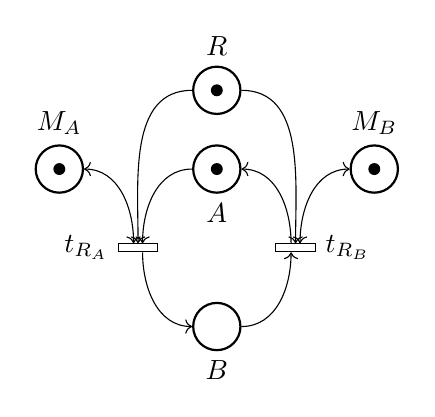
\begin{tikzpicture}
        \node[place,tokens=1,label=above:$M_A$](ma)at(0,0){};
        \node[place,tokens=1,label=above:$R$](r)at(2,1){};
        \node[place,tokens=1,label=above:$M_B$](mb)at(4,0){};
        \node[transition, rotate=90, label=above:$t_{R_A}$](tra)at(1,-1){};
        \node[transition, rotate=90, label=below:$t_{R_B}$](trb)at(3,-1){};

        \draw[<->](ma.0)to[out=0, in=90](tra.45);
        \draw[->](r.180)to[out=180,in=90](tra.0);
        \draw[->](r.0)to[out=0,in=90](trb.0);
        \draw[<->](mb.180)to[out=180, in=90](trb.315);

        \node[place, tokens=1, label=below:$A$](a)at(2,0){};
        \node[place, tokens=0, label=below:$B$](b)at(2,-2){};

        \draw[->](a.180)to[out=180,in=90](tra.315);
        \draw[->](tra.225)to[out=270,in=180](b.180);
        \draw[->](b.0)to[out=0,in=270](trb.135);
        \draw[->](trb.45)to[out=90,in=0](a.0);
    \end{tikzpicture}
\end{center}

In caso $R$ abiliti solo queste due transizioni, si può omettere. Quando si modella l'alternanza, le transizioni possono scattare solo in questo ordine prestabilito, anche 
indipendentemente dalla disponibilità di $M_{A/B}$. Per cui questo metodo di risoluzione di un conflitto è inefficiente. 

Si definisce un nuovo tipo di connesione tra posto e transizioni, detto arco inibitore, questo arco, uscente da un posto, si collega ad una transizione mediante una punta di 
freccia circolare. Se la marca presente nel posto è maggiore uguale al peso $k$ dell'arco inibitore, allora la transizione collegata non può scattare, anche se è abilitata. 
\begin{center}
    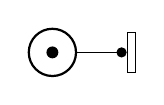
\begin{tikzpicture}
        \node[place, tokens=1](p)at(0,0){};
        \node[transition](t)at(1,0){};

        \draw[-{Circle[]}](p.0)--(t.180);
    \end{tikzpicture}
\end{center}
In questo caso la transizione non può scattare. In questo modo si può risolvere un conflitto tra due transizioni. Una transizione ha priorità sull'altra, quindi si include 
un arco inibitore, di peso pari al peso dell'arco entrante nella transizione che ha priorità. In questo modo solo se la prima transizione non è abilitata, la seconda è in 
grado di scattare:
\begin{center}
    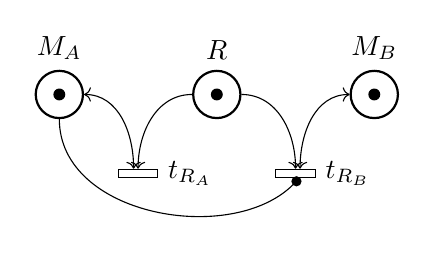
\begin{tikzpicture}
        \node[place,tokens=1,label=above:$M_A$](ma)at(0,0){};
        \node[place,tokens=1,label=above:$R$](r)at(2,0){};
        \node[place,tokens=1,label=above:$M_B$](mb)at(4,0){};
        \node[transition, rotate=90, label=below:$t_{R_A}$](tra)at(1,-1){};
        \node[transition, rotate=90, label=below:$t_{R_B}$](trb)at(3,-1){};

        \draw[<->](ma.0)to[out=0, in=90](tra.45);
        \draw[->](r.180)to[out=180,in=90](tra.0);
        \draw[->](r.0)to[out=0,in=90](trb.0);
        \draw[<->](mb.180)to[out=180, in=90](trb.315);

        \draw[-{Circle[]}](ma.270)to[out=270,in=225](trb.225);
    \end{tikzpicture}
\end{center}
In questo modo non si spreca del tempo ad aspettare che la seconda transizione sia abilitata. Questo metodo di risoluzione è più efficiente rispetto alla priorità. 

Se non viene esplicitamente richiesto, non si modella la risoluzione del conflitto, se invece si modella la risoluzione si usano direttamente le transizioni temporizzate. 

\subsection{Buffer FIFO e LIFO}

In caso il sistema presenta una pila o una coda, bisogna modellare un magazzino con disciplina FIFO o LIFO. 
Si modella un buffer nella convenzione First In First Out, tramite archi inibitori, dove la transizione $t_{out}$ determina l'uscita dell'elemento dal buffer. Si 
considera un buffer di $n$ elementi: 
\begin{center}
    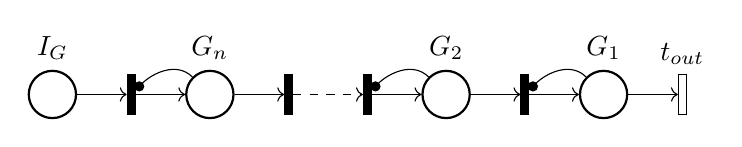
\begin{tikzpicture}
        \node[place,label=above:$I_G$](r)at(-1,0){};
        \node[instant](tp)at(0,0){};
        \node[place,label=above:$G_n$](p0)at(1,0){};
        \node[instant](ta)at(2,0){};

        \node[instant](t1)at(3,0){};
        \node[place,label=above:$G_2$](p1)at(4,0){};
        \node[instant](t2)at(5,0){};
        \node[place,label=above:$G_1$](p2)at(6,0){};
        \node[transition,label=above:$t_{out}$](t0)at(7,0){};

        \draw[->](r.0)--(tp.180);
        \draw[->](tp.0)--(p0.180);
        \draw[->](p0.0)--(ta.180);
        \draw[->](t1.0)--(p1.180);
        \draw[->](p1.0)--(t2.180);
        \draw[->](t2.0)--(p2.180);
        \draw[->](p2.0)--(t0.180);


        \draw[-{Circle[]}](p0.135)to[out=135,in=45](tp.45);
        \draw[-{Circle[]}](p2.135)to[out=135,in=45](t2.45);
        \draw[-{Circle[]}](p1.135)to[out=135,in=45](t1.45);
        \draw[dashed,->](ta.0)--(t1.180);
    \end{tikzpicture}
\end{center}

Si modella ora un buffer LIFO, di $n$ elementi:
\begin{center}
    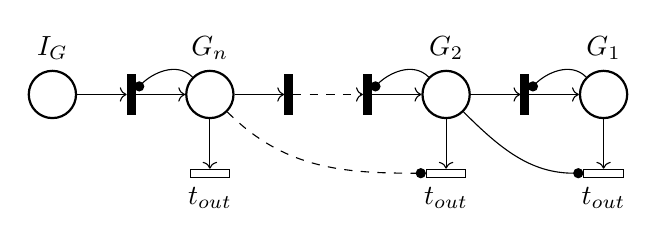
\begin{tikzpicture}
        \node[place,label=above:$I_G$](r)at(-1,0){};
        \node[instant](tp)at(0,0){};
        \node[place,label=above:$G_n$](p0)at(1,0){};
        \node[instant](ta)at(2,0){};
        \node[transition,rotate=90,label=left:$t_{out}$](t00)at(1,-1){};
        \node[instant](t1)at(3,0){};
        \node[place,label=above:$G_2$](p1)at(4,0){};
        \node[instant](t2)at(5,0){};
        \node[transition,rotate=90,label=left:$t_{out}$](t01)at(4,-1){};
        \node[place,label=above:$G_1$](p2)at(6,0){};
        \node[transition,rotate=90,label=left:$t_{out}$](t02)at(6,-1){};

        \draw[->](r.0)--(tp.180);
        \draw[->](tp.0)--(p0.180);
        \draw[->](p0.0)--(ta.180);
        \draw[->](t1.0)--(p1.180);
        \draw[->](p1.0)--(t2.180);
        \draw[->](t2.0)--(p2.180);
        \draw[->](p0.270)--(t00.0);
        \draw[->](p1.270)--(t01.0);
        \draw[->](p2.270)--(t02.0);

        \draw[dashed,-{Circle[]}](p0.315)to[out=315,in=180](t01.90);
        \draw[-{Circle[]}](p1.315)to[out=315,in=180](t02.90);

        \draw[-{Circle[]}](p0.135)to[out=135,in=45](tp.45);
        \draw[-{Circle[]}](p2.135)to[out=135,in=45](t2.45);
        \draw[-{Circle[]}](p1.135)to[out=135,in=45](t1.45);
        \draw[dashed,->](ta.0)--(t1.180);
    \end{tikzpicture}
\end{center}

\subsection{Diagramma di Gant}

Il grafico di Gant è una rappresentazione grafica dell'uso delle risorse in un sistema. Ogni risorsa si indica come una linea parallela. Si scorrono verso destra, rispetto 
al tempo, e viene associato un evento in un determianto tempo per ogni scatto di una o più transizioni. Si può identificare nel grafico di Gant quando è presente un conflitto, 
ovvero quando una stessa risorsa è richiesta per due, o più, processi diversi. Il grafico di Gant è completamente indipendente dalla rete associata ad un sistema. Attraverso 
questa visualizzazione, si possono individuare tutti i conflitti effettivi della rete, quindi si possono modellare adeguatamente le risoluzioni, se sono richieste. La 
precedenza nel grafico di Gant viene scelta arbitrariamente. Questa 
rappresentazione dipende dalla marcatura iniziale del sistema, in caso sia presente un deadlock, la rappresentazione non è periodica. Generalmente un grafico di Gant di un 
sistema produttivo ciclico, è periodico, per cui è sufficiente rappresentare solo un periodo del sistema. 
%% esempio grafo (2/11)

\subsection{Scambio}

Un sistema può arrivare ad una situazione dove due processi sono bloccati, poiché richiedono alcune risorse usate nell'altro processo. Se il sistema si blocca se incontra 
questa situazione, è necessario modellare un metodo in modo in cui il sistema posso continuare ad operare, anche se ragiunta questa situazione. Per modellarlo, bisogna 
dare priorità ad uno dei processi, e si evita di richiedere la disponibilità della risorsa scambiandola con l'altro processo, e riportando quel processo ad uno stato 
precedente all'uso della risorsa. 

\begin{center}
    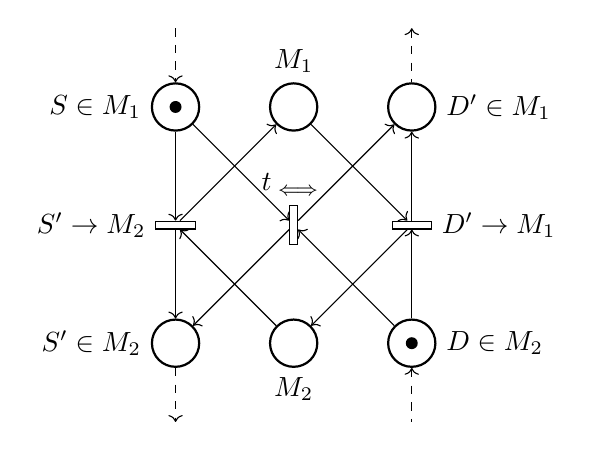
\begin{tikzpicture}
        \node[place,tokens=1,label=left:$S\in M_1$](p1)at(0,3){};
        \node[place,label=right:$ D'\in M_1$](p3)at(3,3){};
        \node[place,label=left:$S'\in M_2$](p2)at(0,0){};
        \node[place,tokens=1,label=right:$ D\in M_2$](p4)at(3,0){};
        \node[place,label=above:$M_1$](m1)at(1.5,3){};
        \node[place,label=below:$M_2$](m2)at(1.5,0){};
        \node[transition,rotate=90,label=above:$ S'\to M_2$](t1)at(0,1.5){};
        \node[transition,rotate=90,label=below:$D'\to M_1$](t2)at(3,1.5){};
        \node[transition, label=above:$t_{\iff}$](t3)at(1.5,1.5){};

        \draw[->](p1.270)--(t1.0);
        \draw[->](t1.180)--(p2.90);
        \draw[<-](p3.270)--(t2.0);
        \draw[<-](t2.180)--(p4.90);
        
        \draw[->](p1.315)--(t3.135);
        \draw[->](t3.45)--(p3.225);
        \draw[->](p4.135)--(t3.315);
        \draw[->](t3.225)--(p2.45);

        \draw[->,dashed](0,4)--(p1.90);
        \draw[<-,dashed](3,4)--(p3.90);
        \draw[->,dashed](p2.270)--(0,-1);
        \draw[<-,dashed](p4.270)--(3,-1);

        \draw[->](t1.315)--(m1.225);
        \draw[->](m1.315)--(t2.45);
        \draw[<-](t1.225)--(m2.135);
        \draw[<-](m2.45)--(t2.135);
    \end{tikzpicture}
\end{center}
In questo esempio è presente una lavorazione in parallelo di due materiali $S$ e $D$, con delle macchine $M_1$ e $M_2$. Nella sequenza di destra, è stata 
usata la risorsa $M_1$, e per continuare la lavorazione è necessaria la risorsa $M_2$, impegnata nella 
lavorazione di destra. Le risorse $M_1$ ed $M_2$, sono entrambe non 
disponibili per entrambe le sequenza, per cui ci si trova in un deadlock. Si prioritizza la lavorazione di sinistra, 
per cui si inserisce una transizione $t_{\iff}$ che evita la richiesta delle due risorse entrambe occupate. 
Dando priorità alla lavorazione di sinistra, il processo di destra, arriva da $ D\in M_2$ ad uno stato $ D'\in M_1$ senza dover 
richiedere la risorsa $M_1$ tramite la transizione $ D'\to M_1$. Mentre il processo di sinistra, arriva da $S\in M_2$ ad uno stato $S'\in M_1$ dove ha già 
richiesto ed ottenuto la risorsa $M_1$, senza lo scatto della transizione $S'\to M_2$, effettivamente scambiando la risorsa tra i due processi. 

\subsection{Contatore}

In alcuni sistemi, un processo può essere attivato solo dopo avere almeno $n$ elementi disponibili. Per modellarlo è necessario un contatore, che si aggiorni per ogni 
nuovo elemento, fino alla raggiunta degli $n$ elementi necessari. Per modellare questo contatore, sono necessari $n+1$ posti, che rappresentano il numero di 
elementi disponibili dal posto $G_0$, che indica non sono presenti elementi, fino al posto $G_{\geq n}$, che indica sono presenti almeno $n$ elementi. Inoltre è necessario un 
qualche tipo di generatore, per poter modellare l'entrata degli elementi nel sistema, ogni intervallo di tempo. Poiché se fossero sempre disponibili non sarebbe necessario 
un contatore. 

\begin{center}
    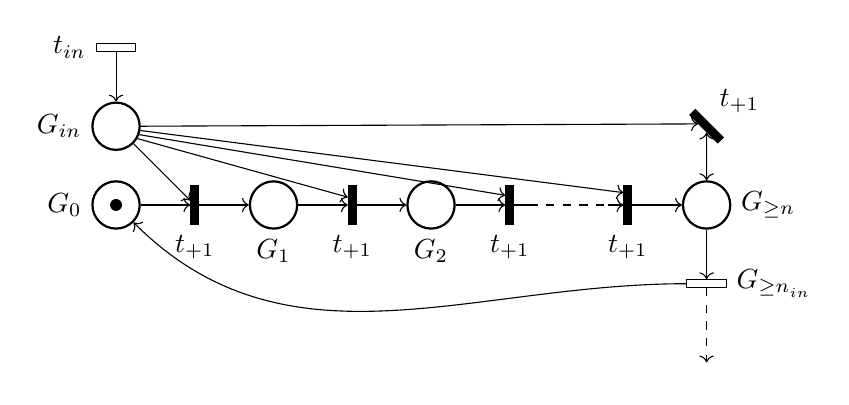
\begin{tikzpicture}
        \node[transition, rotate=90, label=above:$t_{in}$](tin)at(0,2){};
        \node[place, label=left:$G_{in}$](gin)at(0,1){};
        \draw[->](tin.180)--(gin.90);

        \node[place, tokens=1, label=left:$G_0$](g0)at(0,0){};
        \node[instant, label=below:$t_{+1}$](t1)at(1,0){};
        \node[place, label=below:$G_1$](g1)at(2,0){};
        \node[instant, label=below:$t_{+1}$](t2)at(3,0){};
        \node[place, label=below:$G_2$](g2)at(4,0){};
        \node[instant, label=below:$t_{+1}$](t3)at(5,0){};
        \node[instant, label=below:$t_{+1}$](t4)at(6.5,0){};
        \node[place, label=right:$G_{\geq n}$](gn)at(7.5,0){};
        \draw[-](t3.0)--(5.25,0);
        \draw[dashed](5.25,0)--(6.25,0);
        \draw[->](6.25,0)--(t4.180);

        \draw[->](gin.315)--(t1.135);
        \draw[->](g0.0)--(t1.180);
        \draw[->](t1.0)--(g1.180);
        \draw[->](gin.330)--(t2.120);
        \draw[->](g1.0)--(t2.180);
        \draw[->](t2.0)--(g2.180);
        \draw[->](gin.340)--(t3.115);
        \draw[->](g2.0)--(t3.180);
        \draw[->](t4.0)--(gn.180);
        \draw[->](gin.350)--(t4.110);

        \node[transition, rotate=90, label=below:$G_{{\geq n}_{in}}$](tgin)at(7.5,-1){};
        \draw[->](gn.270)--(tgin.0);
        \draw[->](tgin.90)to[out=180,in=315](g0.315);
        \draw[->,dashed](tgin.180)--(7.5,-2);

        \node[instant, rotate=45,label=right:$t_{+1}$](tt)at(7.5,1){};
        \draw[->](gin.0)--(tt.120);
        \draw[<->](tt.225)--(gn.90);
    \end{tikzpicture}
\end{center}


\end{document}